\documentclass[a4paper]{report}
% \documentclass[a4paper,twoside,openright]{report}
% \documentclass[a4paper]{book}

%% Spanska!
\usepackage[utf8]{inputenc}
\usepackage[T1]{fontenc}    % 8-bit encoding. Acentuados como único caracter.
\usepackage[spanish]{babel}
% \def\spanishoptions{argentina}

%% graphics
\usepackage{graphicx}
\graphicspath{ {./graphs/} }
\usepackage{wrapfig}
\usepackage{tikz}

%% biblatex
\usepackage[style=numeric, backend=biber, sorting= none, url= true, maxnames=20]{biblatex}
\DefineBibliographyStrings{spanish}{}
\usepackage{csquotes}
\usepackage{textgreek} % https://tex.stackexchange.com/questions/107352/non-ascii-characters-in-biblatex 
\addbibresource{sismos.bib}

%% physics
\usepackage[separate-uncertainty=true, locale=FR]{siunitx}

%% vínculos en documento pdf
\usepackage{hyperref}
\usepackage[all]{hypcap}
\hypersetup{
    colorlinks=false    % false:boxedlinks ; true:coloredlinks
}

%% tablas
\usepackage{booktabs}

%% matemática
\usepackage{amsmath} % aligned

%% color text
\usepackage{xcolor}



\begin{document}

%\title{
%	{Factores físicos de los terremotos que influyen en su percepción por la población}\\[1 cm]
%	{Trabajo final de la asignatura ``Taller de tesis''}
%	{
\includegraphics[width=\textwidth]{logos}}
%}
%\author{Víctor A. Bettachini}
%\date{\today}
%\maketitle
%
%\begin{abstract}
%	Niente.
%\end{abstract}


% Title page
\begin{titlepage}
    \centering
    %\vspace*{1in}
    
    \huge\textbf{Predicción de la percepción de sismos por la población a partir de datos básicos de terremotos}
    
    \vspace{0.5in}
		Trabajo final de la asignatura\\``Taller de tesis''\\
    \vspace{0.5in}
		
\includegraphics[width=\textwidth]{logos}\\
    \vspace{0.5in}
    
    \large
    \textbf{Autor:}\\
		Víctor A. Bettachini\\
    \vspace{0.5in}
    \textbf{Fecha:}\\
    \today
    
    \vfill
    \begin{minipage}{0.8\textwidth}
    \begin{abstract}
        Una decena de terremotos se producen en el territorio nacional en forma diaria sin que sean detectados más que por instrumentos.
				Son muy pocos los casos en que las ondas sismicas que estos producen son percibidos por la población.
				Este trabajo busca cuantificar la capacidad de predecir esta eventualidad por dos herramientas de la ciencia de datos usando solo datos básicos de terremotos.
    \end{abstract}
		\end{minipage}
	\end{titlepage}

\tableofcontents

% \mainmatter

\chapter{Introducción}

\section{Contexto y motivación científica}\label{sec:contexto}

Un rápido desprendimiento entre dos fascetas enfrentadas de sendas placas tecnónicas que trabanban mutuamente su desplazamiento relativo produce una rápida liberación de energía que se denomina terremoto.
Esto sucede a cierta profundidad en la corteza terrestre en el punto denominado hipocentro a partir del cual parte de esta energía se encauza como ondas elásticas.
El estudio de estas ondas es el área llamada sismología y de ahí el termino sismo para un evento particular detectado, pero que debiera aclararse si se produjo por un terremoto u otra fuente de ondas \cite[sección 4.1.1]{fowler_solid_1990}.
\begin{wrapfigure}[15]{r}{0.4\textwidth}
  \centering
	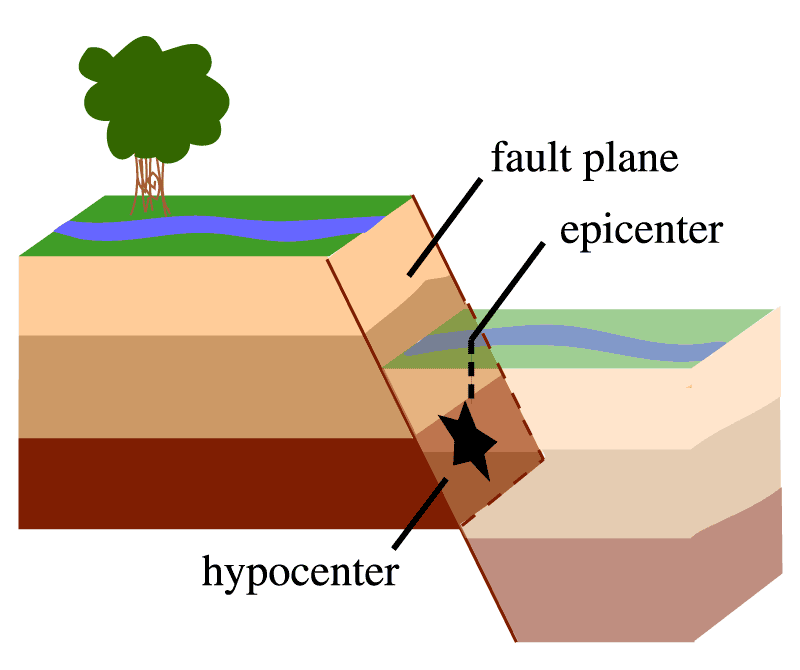
\includegraphics[width=0.4\textwidth]{eq-ed-fault-labeled.png}
	\caption{Epicentro e hipocentro de un sismo.}
	\label{fig:epicentro_hipocentro}
\end{wrapfigure}
Sea que las ondas sean de compresión longitudinal de la corteza, las tipo P, o las del tipo S transversales y más lentas, ambas arriban con mayor intensidad al punto de la superficial terrestre que se encuentra directamente sobre el hipocentro, que se denomina epicentro \cite[sección 4.1.2]{fowler_solid_1990} como ilustra la figura \ref{fig:epicentro_hipocentro}.
Cuanto más proxima es una locación en la superficie a un epicentro la amplitud de las ondas sísmicas es mayor.
Tanto esta amplitud como el período de oscilación son mucho mayores que el de otros desplazamientos de la corteza respecto a otros desplazamientos como los de las mareas solares y lunares de la corteza \cite[sección 4.1.4]{fowler_solid_1990}.
Como resultado estructuras artificiales pueden agitarse poniendo en riesgo su estabilidad estructural y haciendo caer elementos que no estaban fijados a esta o perdieron tal adhesión a causa de la agitación misma.
Como consecuencia los sismos más fuertes pueden generar graves daños, poniendo en riesgo la integridad física y la seguridad de las personas al generar daños en las viviendas y edificios, derrumbes de puentes, rompimiento de vidrios, entre otros \cite{noauthor_que_2018}.

Pero de hecho la mayor parte de los sismos son de muy pequeña magnitud y no generan daños materiales.
Sin embargo el que sean o no detectados por la población es un factor relevante en su percepción de confianza vis-à-vís de los organismos de monitoreo y prevención de riesgos.
Sí o cuando informar a la población de la ocurrencia de un sismo es una decisión de política pública que debiera apuntar a no alertar  innecesariamente sobre sismos menores imperceptibles \cite{saunders_j_k_twist_nodate}.
El caso inverso es también problemático con casos en que ante una carencia de una comunicación oficial de la poca importancia de un evento sismico llevó a la autoevacuación por parte de la población que lo percibió \cite{vaiciulyte_population_2022}. 


\section{Objetivos del trabajo / Pregunta}
Contar con una estimación rápida a partir de los datos sismicos registrados por instrumental de si un dado evento será percibido por la población o no permitiría a las autoridades tomar decisiones informadas sobre la comunicación a la población.
Este trabajo busca determinar el grado de certeza con que ciertos métodos de ciencias de datos pueden predecir si la población percibirá actividad sismica producto de terremotos a partir de unos pocos datos básicos sobre los mismos publicados por el Instituto Nacional de Prevención Sísmica (INPRES) que es el organismo público de Argentina que realiza estudios e investigaciones básicas y aplicadas de sismología \cite{noauthor_instituto_2022}.



\section{Estructura del documento}

Se estructuró en los siguientes capitulos con temáticas difenciadas
\begin{description}
	\item[Introducción]: se presentará el contexto y la motivación científica, los objetivos del trabajo y la estructura del documento.
	\item[Marco teórico]: se revisarán los trabajos previos y relevantes, se presentarán los conceptos y técnicas de ciencia de datos utilizados en el trabajo.
	\item[Metodología]: se describirán los datos utilizados, el preprocesamiento y limpieza de los mismos, el análisis exploratorio de los datos, las técnicas de análisis y modelado utilizadas, la selección de características, las métricas de evaluación de los modelos y los métodos estadísticos utilizados.
	\item[Resultados y discusión]: se presentarán y analizarán los resultados obtenidos, se discutirán los resultados y su relevancia, se identificarán las limitaciones y posibles mejoras.
	\item[Conclusión]: se resumirán los hallazgos principales, se presentarán las conclusiones generales y su relación con los objetivos del trabajo, se discutirán las aplicaciones y relevancia de los resultados.
\end{description}



\chapter{Marco teórico}

\section{Relevamiento de trabajos previos y relevantes}

En relación con la temática de terremotos los trabajos publicados que hacen uso de herramientas de aprendizaje autómático en su mayoría persiguen el esquivo objetivo de predecir la ocurrencia de sismos de gran intensidad, y en segundo lugar para la mejora de la detección de estos por parte de instrumental, pero la temática de la perecpiún de los mismos por humanos no parece ser una temática corriente \cite{hu_applying_2024}.

Un trabajo interesante no porque sea un antecedente del enfoque o temática de este trabajo pero sí por tocar al aspecto social de la percecpión de sismos hace uso del método conocido como SHAP (contracción de SHapley Additive exPlanations, explicaciones aditivas de Shapley) que determina la contribución de cada carecterística en un conjunto de datos a una determinada predicción \cite{molnar_96_2024}.
Los datos son características sociológicas de los individuos y la predicción es sobre la percepción personal del riesgo sismológico.
Los autores muestran un resultado estadístico que avala el que se incrementa la percepción del riesgo de esta fuente tras haber percibido un sismo \cite{bedle_recognizing_2022}.

Un estudio de la problemática de la percecpión por la población de un terremoto tal vez deba separarse en dos problemas a resolver secuencialmente.
En primer lugar determinar el espectro de frecuencias de oscilación del suelo en función de características físicas del terremoto y la corteza.
Y en segundo lugar la respuesta de las personas a tal espectro de oscilaciones que depende además de características de las viviendas más crucialmente de cuestiones fisiológicas.

Atendiendo a la primer cuestión la modelización física ha arribado a un conjunto de ecuaciones para predecir el especto de frecuencias de oscilación del suelo en función de la distancia al hipocentro y las características de la corteza en el camino de propagación de las ondas desde el terremoto \cite{lior_relation_2018}.
Pero como estas ecuaciones dependen de una multitud de factores que deben ajustarse a cada locación en muchos casos en forma empírica se han ensayado alternativas basadas en el aprendizaje autómático en años recientes, en particular utilizando arquitecturas de redes neuroles recurrentes \cite{datta_deepshake_2022}.

En cuanto a la segunda cuestión, la respuesta fisiológica al espectro de oscilaciones del suelo, el foco también a sido el consante en el campo de la sismología, el de la predicción de terremotos de gran importancia.
El campo se ha enfocado primordialmente a la capacidad sensora no de humanos sino de animales tradicionalmente considerados más sensibles y fuentes de señal de alarma ante sismos \cite{kirschvink_earthquake_2000}.

Pero en la superficial búsqueda superficial de literatura realizada para este trabajo no encontré antecedentes que cubrieran todo el arco desde características que describen el terremoto hasta la determinación excluyente de si los correspondientes sismos son o no percibidos por la población.


\section{Conceptos y técnicas de ciencia de datos utilizados en el trabajo}

% Siendo el objetivo de cualquier modelo utilizado una clasificación entre dos clases, la percepción de un sismo o no, se busca determinar que tan fuerte es el vínculo de cada una de las variables de los sismos de las que se dispone datos y la percepción de los mismos por parte de la población.

Se utilizan en este trabajo dos técnicas con aplicación a la predicción pero en sendos extremos de complejidad y transparencia en cuanto al peso relativo que tienen las variables independientes en el resultado, el de regresión logística y el de máquinas de potenciacion de gradiente, más conocidos por su nombre en inglés Gradient Boosting Machines (GBM).


\subsection{Regresión logística para la predicción binaria}

La siguiente es un resumen del material de la novena clase de la asignatua \emph{Enfoque estadístico del aprendizaje} titulada \emph{Regresión Logística} elaborodo por Juan Barriola, Azul Villanueva y Franco Mastelli. 

Un modelo de regresión lineal con coeficientes \(beta_i\) para cada variable \(X_i\) que busque la probabilidad de una dependiente binaria \(P(Y)\)  
\[
P(Y) = \beta_0 + \sum\limits_{j=1}^p \beta_j X_j,	
\]
no presentaría un punto de corte claro para clasificar los datos en dos categorías.
Para sortear esta dificulta se toma la salida de esta regresión como la variable dependiente de una regresión logística,
\[
P(Y|X)= \frac{e^{\beta_0 + \sum\limits_{j=1}^p \beta_j X_j}}{1+e^{\beta_0 + \sum\limits_{j=1}^p \beta_j X_j}},
\]
lo que asegura un valor entre 0 y 1.
De esta expresión puede arribarse a 
\[
	\log {\frac{P(x)}{1-P(x)}}= \beta_0 + \sum\limits_{j=1}^p \beta_j X_j,
\]
cuyo lado izquierdo es el logaritmo de los \emph{odds} y se llama \emph{logit}. 

La funcíón \verb'glm' de la biblioteca \verb'glmnet' permite crear un modelo lineal generalizado (Generalized Linear Model).
Al igual que la función de modelo lineal \verb'lm' toma como argumentos una \emph{formula} y los \emph{datos} pero también se debe especificar el argumento \emph{family}: indicamos la distribución del error y la función link que vamos a utilizar en el modelo según la distribución que corresponde a la variable a predecir 
\begin{itemize}
	\item Binomial: link=logit
	\item Poisson: link=log
	\item Gaussiana: link=identidad
\end{itemize}
Como estamos trabajando con un fenómeno que suponemos tiene una distribución binomial, así lo especificamos en el parámetro \emph{family}.

Aunque se parte de pocas variables independientes, se ensayará forzar una mayor simplificación del mismo mediante la técnica de regularización tipo Lasso (L1) que fuerza a que los coeficientes de las variables independientes que menos aportan a predicción vayan anulándose.


\subsection{XGBoost para una predicción binaria}

En otro extremo entre las herramientas de ciencia de datos por su complijidad se ensayará utilizar máquinas de potenciacion de gradiente, más conocidos por su nombre en inglés Gradient Boosting Machines (GBM) para la predicción
Las distintas implementaciones de estos algoritmos, como XGBoost, LightGBM o CatBoost son capaces de producir un único modelo con fuerte poder predictivo a partir de la síntesis de resultados de modelos de predicción débiles, típicamente árboles de decisión. 
En particular se utiliza la implementación de XGBoost en lenguaje R para este trabajo.

%Puesto que los GBM carecen de un mecanísmo para evidenciar la importancia de las variables en la clasificación como la que evidencian los pesos de la regresión logística, se planea utilizar los valores del método SHAP comentado en la sección anterior para tal fin.
%Para el lenguaje R está disponible la biblioteca \emph{shapr} para tal fin \cite{camilla_lingjaerde_shapr_nodate}.

%El disponer de una herramienta de explicación de los modelos de predección aplicable al resultado de los dos a ensayar, el de regresión lógistica y el XGBoost, permitirá comparar la relevancia de las variables que asignará cada uno para la percepción de los sismos por parte de la población.




\chapter{Metodología}

\section{Presentación y descripción de los datos utilizados}

En el marco de los ``Proyectos de Asistencia Estadística del Instituto de Cálculo (IC)'' de la Facultad de Ciencias Exactas y Naturales (FCEyN) de la Universidad de Buenos Aires (UBA) se publicaron conjuntos de datos en un repositorio curado con el objeto de ser aplicados a la enseñanza de la estadística y la ciencia de datos por Daniela Parada, investigadora del IC \cite{noauthor_ic-datasets-docencia_nodate}.
De estos conjuntos el utilizado en este trabajo es el que se publica en el apartado ``Visualización'' que corresponden a datos de sismos de Argentina de la última década \cite{daniela_parada_ic-datasets-docencia_nodate}. 
En este repositorio alojado por la firma GitHub, se provee un front-end html que da un contexto, hace una exploración inicial, un analísis para una provincia en particular, muestra una estimación de probabilidad y provee otra información sobre lo datos.

Los datos corresponden a detecciones por parte de estaciones de monitoreo sísmico en la República Argentina recopilados y publicados por el INPRES en su sitio web \cite{noauthor_buscador_nodate}.
En el sitio de publicación de los datos se indica que el conjunto de datos comprende las fechas desde el 7 de enero de 2012 hasta el 18 de mayo de 2022 y fue realizado con datos \emph{scrappeados} del buscador de sismos del INPRES por Gustavo Juantorena \cite[sección 4.1]{daniela_parada_ic-datasets-docencia_nodate}. 

Allí mismo se describe que el conjunto de datos reducido y curado denominado ``sismos'', el que se utilizó en este trabajo, es accesible a través de la importación de la biblioteca \texttt{datosIC} en lenguaje R  \cite[sección 5.1.1]{daniela_parada_ic-datasets-docencia_nodate}.
Este mismo conjunto reducido puede descargarse en formato de texto separado por comas (CSV) apuntando a su URL en el repositorio GitHub\footnote{\url{https://github.com/daniellaparada/IC-datasets-docencia/blob/main/fuente/04_visualizacion/sismos-arg.csv}}.

Las variables reportadas para cada sismo son:
\begin{itemize}
	\item \emph{Fecha}: en el formato verb`aaaa-mm-dd`'' de la norma ISO 8601 \cite{noauthor_iso_2019}.
	\item \emph{Hora}: una cadena de caracteres en formato \verb`hh:mm:ss`'' con una exactitud al segundo.
	\item \emph{Latitud, Longitud}: un número con una exactitud de un decimal con grados como unidad.
	\item \emph{Provincia}: cadena de caractéres del nombre de la provincia donde se produjo el sismo (no donde se ubicó quién potencialmente lo percibiera) según se afirma en el sitio de publicación \cite[5.1.1]{daniela_parada_ic-datasets-docencia_nodate}.
	\item \emph{Magnitud}: un número con la escala Richter como unidad una función de la amplitud de las ondas sísmicas \cite[sección 4.2.3]{fowler_solid_1990}
	\item \emph{Profundidad}: un número entero con kilometros como unidad que indico que tan bajo la superficie se ubicó el epicentro.
	\item \emph{Percibido}: variable booleana de si hubo reportes de percepeción del fenómeno por parte de la población, 
\end{itemize}
Esta última variable es la que se busca predecir en este trabajo en función de las demás. 



\section{Limpieza de los datos}

Puesto que el conjunto de datos es curado por un equipo de investigación de la UBA, se asume que los mismos son confiables y que no se requiere de un proceso de limpieza de los mismos.
De todas formas se realizaron las verificaciones usuales cada vez que se utilizan datos tabulares en un estudio de estadístico y/o de ciencia de datos.

\paragraph{Carga de los datos}
Tras descargar el archivo de datos en fomato CSV se le importó en una estructura de datos \emph{data.table} de en un entorno de trabajo en lenguaje R.
Esta estructura de datos permite una consulta de los datos análoga a la del lenguaje SQL de bases de datos relacionales lo que le hace una herramienta versatil para el análisis de datos tabulares \cite{noauthor_introduction_2024}.

\paragraph{Inspección de tipos de datos}
Ejecutar la funcíon \verb'colnames' con la \emph{data.table} denominada \verb'sismos_arg' como argumento permitió verificar que contuviera las columnas con los nombres anunciados en el sitio que publica los datos en su sección \cite[Exploración inicial]{daniela_parada_ic-datasets-docencia_nodate}.
Las transformaciones o ingeniería de características que se detallan luego en esta sección se realizaron en función de los tipos de datos de cada columnas constatados con la función \verb'str'.


\paragraph{Valores faltantes o duplicados}
La presencia de valores faltantes indicados con el símbolo \verb'NA' se descartó cuando la ejecución \verb'sum(is.na(sismos_arg))' arrojó un cero como resultado.
Por el contrario unos \num{23} registros duplicadas mostró
ejecutar \verb'sismos_arg[duplicated(sismos_arg, fromLast = TRUE)]' sobre un total de \num{55817} registros.
Se hizo una copia de la tabla sin registros duplicados ejecutando \verb'sismos_arg[!duplicated(sismos_arg)]' en una nueva tabla con nombre más corto, \verb'sismos'.


\paragraph{Datos atípicos}
La detección y potenciales acciones sobre datos atípicos se tratan una vez iniciado un análisis exploratorio de datos temática de la sección \ref{sec:AED}.



\section{Ingeniería de características}

Por otra parte el preprocesamiento comprende la generación de nuevas variables a partir de las existentes que se consideren relevantes para el análisis, lo que recibe el nombre de ingeniería de características (feature engineering).

Esto comprende tareas de distinta naturaleza.
Por un lado las que se realizan para adecuar el formato de datos para las herramientas a utilizar como el que se describe en el próximo párrafo.
Otras de estas es una modificación basada en un conocimiento del sistema que genera los datos.
En estos casos se hace uso de un críterio que parte de condicionamientos sobre el sistema físico o se implementa un modelo en base a la física del sistema.
Dos de las variables de este conjunto de datos son afectadas por este tipo de modificación, que se decribe posteriormente en una subsección.

% Se generaron dos nuevas columnas a partir de las existentes en el conjunto de datos original, una en función al formato de los datos en la columna \verb'Hora' y otra en función de la escala física utilizada en la columna \verb'Magnitud'.


\paragraph{Decimalización de la hora del sismo}
La columna ``Hora'' está codificada como una cadena de caracteres.
Para poder utilizarla en un análisis de regresión se la convirtió a un número entero de segundos transcurridos desde la medianoche del día en que se produjo el sismo. 
Para ello se escribió una función \verb'convert_to_seconds' centrada en la función \verb'strptime' del paquete base de R.
Se verificó que la columna generada con aplicación a través de \verb'sismos[, Hora_decimal := sapply(Hora, convert_to_seconds)]' estuvieron en el rango de \num{0} a \SI{86400}{\second}, es decir, el de un día completo.


\subsection{Modificaciones inspiradas en la física del sistema}
% \section{Descripción de las técnicas de análisis y, si corresponde, de modelado}


\paragraph{Recorte por profundidad}

Puesto que hay sismos que no tienen origen en terromotos.
Pueden tener origen en desplazamientos superficiales de tierra, explosiones para la minera o el fracturado hidráulico para la extracción de hidrocarburos.
Se busca omitir tales origenes en los datos informados.

\begin{wrapfigure}[17]{r}{0.4\textwidth}
	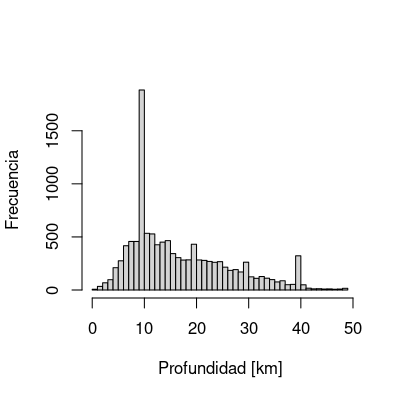
\includegraphics[width=0.4\textwidth]{histograma_profundidad_menos50.png}
	\caption{Los sismos con produndidad de \SI{0}{km} son pocos.}
	\label{fig:histograma_profundidad}
\end{wrapfigure}
Con ese fin se decidió trabajar solo con los sismos que se originaron a una profundidad mayor a \SI{0}{\kilo\metre} filtrando con \verb'sismos <- sismos[Profundidad > 0]'.

Siendo que la variable se informa como enteros de kilometros, estos representarían los hipocentros hasta una profundidad de \SI{500}{\metre}, compatibles con estas actividades artificiales.
Esta es una práctica usual en el análisis de datos orientados a sismos originados en terremotos \cite{hu_applying_2024}.
Esto es un número muy pequeño de los sismos en el conjunto de datos como la muestra el histograma según su profundidad que reproduce la figura \ref{fig:histograma_profundidad}.


\paragraph{Linealización de la magnitud}
Todas las escalas de magnitud de los sismos son logarítmicas con una forma genérica
\begin{equation}
	M = \log_{10} \left( \frac{A}{T} \right) + q(\Delta, h) + a,
	\label{eq:magnitud}
\end{equation}
donde \(M\) es la magnitud, \(A\) es la amplitud de las ondas, \(T\) es el período de oscilación, \(q\) es una función de ajuste para el ángulo desde la vertical desde el sismógrafo al \(\Delta\) y su profundidad \(h\), y \(a\) es una constante de ajuste \cite[ecuación 4.13]{fowler_solid_1990}.
Son las ondas S y P (ver sección \ref{sec:contexto}) tienen distintos coeficientes de ajuste en la ecuación \ref{eq:magnitud} y por ello se utilizan distintas escalas de magnitud.
La más generalmente usada hay día es la de Gutemberg-Richter publicada en 1956 para la magnitud de este tipo de ondas, \(m_b\) ,
\begin{equation}
	m_b = \log_{10} \left( \frac{A}{T} \right)_\text{máx} + q(\Delta, h),
	\label{eq:richter}
\end{equation}
sin la constante de ajuste \(a\) y con valores de \(q(\Delta, h)\) en un rango \(\approx \SIrange{6}{8}{}\)  para ondas P en \(\Delta = \SIrange{10}{110}{} ^\circ\) \cite[ecuación 4.18]{fowler_solid_1990}.
Entonces la escala de Gutember-Richter de un terremoto es el logaritmo en base \num{10} de la mayor razón de la amplitud y período de las ondas registradas por los sismógrafos incluyendo ajustes para compensar la variación en la distancia entre el sismógrafo y el hipocentro \cite{willian_l_ellsworth_earthquake_1991}.

Puesto que la magnitud busca dar cuenta de la energía liberada en el terremoto pero este trabajo busca predecir la percepción de los sismos, es de interés obtener un valor que sea lineal con la amplitud registrada por los sismógrafos en superficie, \(A\), que también es la que afecta a las personas. 
Para obtener un valor lineal con esta \(A\) a partir de los datos de magnitud del INPRES se consideró usar una valor medio del rango comentado en el párrafo anterior, \(\overline{q}(\Delta,h)\), con lo que podría despejarse
\begin{equation}
	\left( \frac{A}{T} \right)_\text{máx} = 10^{(m_b - \overline{q}(\Delta,h) )}.
	\label{eq:linealizacionMagnitud}
\end{equation}
Pero si se toma tal promedio se establecería un \(\overline{q}(\Delta,h) = 7\), que cuasará que haya valores negativos para el valor a la izquierda de la ecuación pues el menor \(m_b\) en el conjunto de datos es \num{2.5}, y ese sería algo sin validez física (¡amplitudes negativas!).
Se utilizará entonces este último como valor para \(q(\Delta,h)\).  

De querer despejar la amplitud de las ondas, \(A\), debe establecerse que hacer con el período de las ondas, \(T\), dato que no figura en el conjunto de datos.
No se encontró otra alternativa que asumir que todos los fenómenos registrados tienen el mismo y en consecuecia asumir \(T_\text{consante}\).
Así realizando despejes a partir de la ecuación \ref{eq:richter} asumiendo tales condicionantes todo cuanto puede aproximarse a un valor relacionado la amplitud será una lineal con registrada por un sismógrafo, \(A_\text{máx}\),
\begin{equation}
	\left( \frac{A_\text{máx}}{T_\text{constante}} \right) = 10^{(m_b - 2.5)}.
	\label{eq:linealizacionMagnitud_final} 
\end{equation}
Con el comando \verb'sismos[, proxy_amplitud := 10^(Magnitud- 2.5)]' se generó una columna para este valor denominada \verb'proxy_amplitud'.



\section{Análisis exploratorio de datos (AED)}\label{sec:AED}

Un primer vistazo sobre los datos con \verb'summary(sismos)' permitió obtener un resumen de las variables numéricas y categóricas.
Saltan a la vista que hay valores extremos en la variable \verb'Magnitud' y un fuerte desbalance en la variable ``Percibido'', la de clase de clasificación.


\paragraph{Desbalance de la clase de clasificación}
Sobre el total de 55794 registros únicos, un \(\approx 96.6\%\) solo fueron percibidos por el instrumental y no por la población.
Restan tan solo unos 1905 registros, un \(\approx 3.4\%\), que si fueron percibidos por la población.
Este desbalance llama al uso de técnicas de balanceo de clases en los modelos de clasificación a utilizar.


\paragraph{Distribución de la magnitud}
La magnitud de terremotos forzosamente presenta una distribución asimétrica por el hecho de que cuanto mayor es la energía liberada, más infrecuente es el fenómeno.
Esto la ilustra el número por año de sismos representado en una esacala logarítmica en función de la magnitud generado con código provisto junto con los datos \cite[sección 4.2.1]{daniela_parada_ic-datasets-docencia_nodate}, que se reproduce en la figura \ref{fig:acumulado_anual_magnitud}.

%\begin{figure}[h]
%% \begin{wrapfigure}[13]{r}{0.5\textwidth}
%\centering
%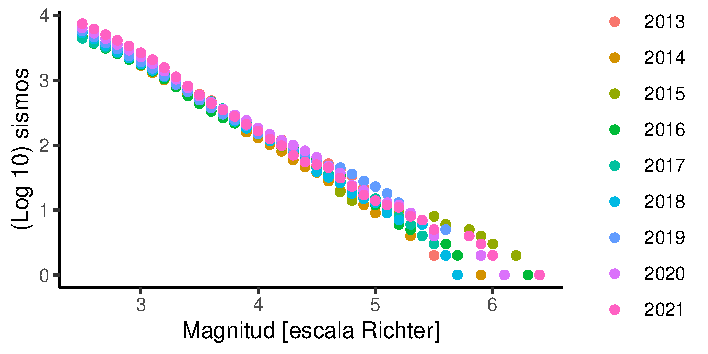
\includegraphics{acumulado_anual_magnitud.pdf}
%% 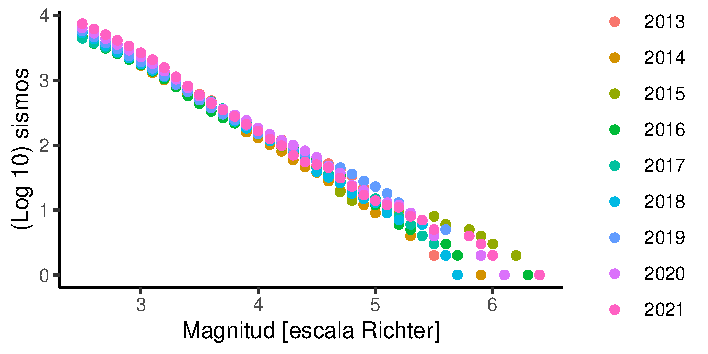
\includegraphics[width=0.5\textwidth]{acumulado_anual_magnitud.pdf}
%\caption{Los sismos de mayor magnitud son más infrecuentes.}
%\label{fig:acumulado_anual_magnitud}
%% \end{wrapfigure}
%\end{figure}

\begin{figure}[!h]
\centering
% The output from tikz()
% is imported here.
% Created by tikzDevice version 0.12.6 on 2024-07-04 02:45:07
% !TEX encoding = UTF-8 Unicode
\begin{tikzpicture}[x=1pt,y=1pt]
\definecolor{fillColor}{RGB}{255,255,255}
\path[use as bounding box,fill=fillColor,fill opacity=0.00] (0,0) rectangle (361.35,216.81);
\begin{scope}
\path[clip] (  0.00,  0.00) rectangle (361.35,216.81);
\definecolor{drawColor}{RGB}{255,255,255}
\definecolor{fillColor}{RGB}{255,255,255}

\path[draw=drawColor,line width= 0.6pt,line join=round,line cap=round,fill=fillColor] (  0.00,  0.00) rectangle (361.35,216.81);
\end{scope}
\begin{scope}
\path[clip] ( 27.31, 30.69) rectangle (296.30,211.31);
\definecolor{fillColor}{RGB}{255,255,255}

\path[fill=fillColor] ( 27.31, 30.69) rectangle (296.30,211.31);
\definecolor{drawColor}{RGB}{248,118,109}
\definecolor{fillColor}{RGB}{248,118,109}

\path[draw=drawColor,line width= 0.4pt,line join=round,line cap=round,fill=fillColor] (208.83, 38.90) circle (  1.96);

\path[draw=drawColor,line width= 0.4pt,line join=round,line cap=round,fill=fillColor] (202.56, 52.59) circle (  1.96);

\path[draw=drawColor,line width= 0.4pt,line join=round,line cap=round,fill=fillColor] (183.75, 60.60) circle (  1.96);

\path[draw=drawColor,line width= 0.4pt,line join=round,line cap=round,fill=fillColor] (177.48, 70.69) circle (  1.96);

\path[draw=drawColor,line width= 0.4pt,line join=round,line cap=round,fill=fillColor] (171.21, 86.27) circle (  1.96);

\path[draw=drawColor,line width= 0.4pt,line join=round,line cap=round,fill=fillColor] (164.94, 94.87) circle (  1.96);

\path[draw=drawColor,line width= 0.4pt,line join=round,line cap=round,fill=fillColor] (158.67,100.84) circle (  1.96);

\path[draw=drawColor,line width= 0.4pt,line join=round,line cap=round,fill=fillColor] (152.40,106.74) circle (  1.96);

\path[draw=drawColor,line width= 0.4pt,line join=round,line cap=round,fill=fillColor] (146.13,112.74) circle (  1.96);

\path[draw=drawColor,line width= 0.4pt,line join=round,line cap=round,fill=fillColor] (139.86,118.77) circle (  1.96);

\path[draw=drawColor,line width= 0.4pt,line join=round,line cap=round,fill=fillColor] (133.59,125.47) circle (  1.96);

\path[draw=drawColor,line width= 0.4pt,line join=round,line cap=round,fill=fillColor] (127.32,129.48) circle (  1.96);

\path[draw=drawColor,line width= 0.4pt,line join=round,line cap=round,fill=fillColor] (121.05,135.21) circle (  1.96);

\path[draw=drawColor,line width= 0.4pt,line join=round,line cap=round,fill=fillColor] (114.78,140.12) circle (  1.96);

\path[draw=drawColor,line width= 0.4pt,line join=round,line cap=round,fill=fillColor] (108.51,145.72) circle (  1.96);

\path[draw=drawColor,line width= 0.4pt,line join=round,line cap=round,fill=fillColor] (102.24,151.91) circle (  1.96);

\path[draw=drawColor,line width= 0.4pt,line join=round,line cap=round,fill=fillColor] ( 95.97,157.21) circle (  1.96);

\path[draw=drawColor,line width= 0.4pt,line join=round,line cap=round,fill=fillColor] ( 89.70,162.71) circle (  1.96);

\path[draw=drawColor,line width= 0.4pt,line join=round,line cap=round,fill=fillColor] ( 83.43,168.29) circle (  1.96);

\path[draw=drawColor,line width= 0.4pt,line join=round,line cap=round,fill=fillColor] ( 77.16,173.44) circle (  1.96);

\path[draw=drawColor,line width= 0.4pt,line join=round,line cap=round,fill=fillColor] ( 70.89,177.99) circle (  1.96);

\path[draw=drawColor,line width= 0.4pt,line join=round,line cap=round,fill=fillColor] ( 64.62,182.85) circle (  1.96);

\path[draw=drawColor,line width= 0.4pt,line join=round,line cap=round,fill=fillColor] ( 58.35,186.71) circle (  1.96);

\path[draw=drawColor,line width= 0.4pt,line join=round,line cap=round,fill=fillColor] ( 52.08,190.36) circle (  1.96);

\path[draw=drawColor,line width= 0.4pt,line join=round,line cap=round,fill=fillColor] ( 45.81,193.56) circle (  1.96);

\path[draw=drawColor,line width= 0.4pt,line join=round,line cap=round,fill=fillColor] ( 39.54,196.26) circle (  1.96);
\definecolor{drawColor}{RGB}{219,142,0}
\definecolor{fillColor}{RGB}{219,142,0}

\path[draw=drawColor,line width= 0.4pt,line join=round,line cap=round,fill=fillColor] (221.37, 38.90) circle (  1.96);

\path[draw=drawColor,line width= 0.4pt,line join=round,line cap=round,fill=fillColor] (215.10, 52.59) circle (  1.96);

\path[draw=drawColor,line width= 0.4pt,line join=round,line cap=round,fill=fillColor] (202.56, 60.60) circle (  1.96);

\path[draw=drawColor,line width= 0.4pt,line join=round,line cap=round,fill=fillColor] (196.29, 70.69) circle (  1.96);

\path[draw=drawColor,line width= 0.4pt,line join=round,line cap=round,fill=fillColor] (190.02, 77.34) circle (  1.96);

\path[draw=drawColor,line width= 0.4pt,line join=round,line cap=round,fill=fillColor] (183.75, 84.39) circle (  1.96);

\path[draw=drawColor,line width= 0.4pt,line join=round,line cap=round,fill=fillColor] (177.48, 87.99) circle (  1.96);

\path[draw=drawColor,line width= 0.4pt,line join=round,line cap=round,fill=fillColor] (171.21, 89.57) circle (  1.96);

\path[draw=drawColor,line width= 0.4pt,line join=round,line cap=round,fill=fillColor] (164.94, 93.67) circle (  1.96);

\path[draw=drawColor,line width= 0.4pt,line join=round,line cap=round,fill=fillColor] (158.67, 98.08) circle (  1.96);

\path[draw=drawColor,line width= 0.4pt,line join=round,line cap=round,fill=fillColor] (152.40,105.42) circle (  1.96);

\path[draw=drawColor,line width= 0.4pt,line join=round,line cap=round,fill=fillColor] (146.13,110.23) circle (  1.96);

\path[draw=drawColor,line width= 0.4pt,line join=round,line cap=round,fill=fillColor] (139.86,115.37) circle (  1.96);

\path[draw=drawColor,line width= 0.4pt,line join=round,line cap=round,fill=fillColor] (133.59,119.78) circle (  1.96);

\path[draw=drawColor,line width= 0.4pt,line join=round,line cap=round,fill=fillColor] (127.32,122.83) circle (  1.96);

\path[draw=drawColor,line width= 0.4pt,line join=round,line cap=round,fill=fillColor] (121.05,129.68) circle (  1.96);

\path[draw=drawColor,line width= 0.4pt,line join=round,line cap=round,fill=fillColor] (114.78,134.75) circle (  1.96);

\path[draw=drawColor,line width= 0.4pt,line join=round,line cap=round,fill=fillColor] (108.51,141.81) circle (  1.96);

\path[draw=drawColor,line width= 0.4pt,line join=round,line cap=round,fill=fillColor] (102.24,147.42) circle (  1.96);

\path[draw=drawColor,line width= 0.4pt,line join=round,line cap=round,fill=fillColor] ( 95.97,152.98) circle (  1.96);

\path[draw=drawColor,line width= 0.4pt,line join=round,line cap=round,fill=fillColor] ( 89.70,158.13) circle (  1.96);

\path[draw=drawColor,line width= 0.4pt,line join=round,line cap=round,fill=fillColor] ( 83.43,163.80) circle (  1.96);

\path[draw=drawColor,line width= 0.4pt,line join=round,line cap=round,fill=fillColor] ( 77.16,169.09) circle (  1.96);

\path[draw=drawColor,line width= 0.4pt,line join=round,line cap=round,fill=fillColor] ( 70.89,174.33) circle (  1.96);

\path[draw=drawColor,line width= 0.4pt,line join=round,line cap=round,fill=fillColor] ( 64.62,178.38) circle (  1.96);

\path[draw=drawColor,line width= 0.4pt,line join=round,line cap=round,fill=fillColor] ( 58.35,182.42) circle (  1.96);

\path[draw=drawColor,line width= 0.4pt,line join=round,line cap=round,fill=fillColor] ( 52.08,186.48) circle (  1.96);

\path[draw=drawColor,line width= 0.4pt,line join=round,line cap=round,fill=fillColor] ( 45.81,189.73) circle (  1.96);

\path[draw=drawColor,line width= 0.4pt,line join=round,line cap=round,fill=fillColor] ( 39.54,192.64) circle (  1.96);
\definecolor{drawColor}{RGB}{174,162,0}
\definecolor{fillColor}{RGB}{174,162,0}

\path[draw=drawColor,line width= 0.4pt,line join=round,line cap=round,fill=fillColor] (233.91, 38.90) circle (  1.96);

\path[draw=drawColor,line width= 0.4pt,line join=round,line cap=round,fill=fillColor] (215.10, 52.59) circle (  1.96);

\path[draw=drawColor,line width= 0.4pt,line join=round,line cap=round,fill=fillColor] (196.29, 60.60) circle (  1.96);

\path[draw=drawColor,line width= 0.4pt,line join=round,line cap=round,fill=fillColor] (183.75, 70.69) circle (  1.96);

\path[draw=drawColor,line width= 0.4pt,line join=round,line cap=round,fill=fillColor] (177.48, 77.34) circle (  1.96);

\path[draw=drawColor,line width= 0.4pt,line join=round,line cap=round,fill=fillColor] (171.21, 82.30) circle (  1.96);

\path[draw=drawColor,line width= 0.4pt,line join=round,line cap=round,fill=fillColor] (158.67, 86.27) circle (  1.96);

\path[draw=drawColor,line width= 0.4pt,line join=round,line cap=round,fill=fillColor] (152.40, 93.67) circle (  1.96);

\path[draw=drawColor,line width= 0.4pt,line join=round,line cap=round,fill=fillColor] (146.13,101.68) circle (  1.96);

\path[draw=drawColor,line width= 0.4pt,line join=round,line cap=round,fill=fillColor] (139.86,108.56) circle (  1.96);

\path[draw=drawColor,line width= 0.4pt,line join=round,line cap=round,fill=fillColor] (133.59,114.10) circle (  1.96);

\path[draw=drawColor,line width= 0.4pt,line join=round,line cap=round,fill=fillColor] (127.32,118.06) circle (  1.96);

\path[draw=drawColor,line width= 0.4pt,line join=round,line cap=round,fill=fillColor] (121.05,123.39) circle (  1.96);

\path[draw=drawColor,line width= 0.4pt,line join=round,line cap=round,fill=fillColor] (114.78,129.68) circle (  1.96);

\path[draw=drawColor,line width= 0.4pt,line join=round,line cap=round,fill=fillColor] (108.51,134.28) circle (  1.96);

\path[draw=drawColor,line width= 0.4pt,line join=round,line cap=round,fill=fillColor] (102.24,140.70) circle (  1.96);

\path[draw=drawColor,line width= 0.4pt,line join=round,line cap=round,fill=fillColor] ( 95.97,146.16) circle (  1.96);

\path[draw=drawColor,line width= 0.4pt,line join=round,line cap=round,fill=fillColor] ( 89.70,152.48) circle (  1.96);

\path[draw=drawColor,line width= 0.4pt,line join=round,line cap=round,fill=fillColor] ( 83.43,157.89) circle (  1.96);

\path[draw=drawColor,line width= 0.4pt,line join=round,line cap=round,fill=fillColor] ( 77.16,163.66) circle (  1.96);

\path[draw=drawColor,line width= 0.4pt,line join=round,line cap=round,fill=fillColor] ( 70.89,169.84) circle (  1.96);

\path[draw=drawColor,line width= 0.4pt,line join=round,line cap=round,fill=fillColor] ( 64.62,175.72) circle (  1.96);

\path[draw=drawColor,line width= 0.4pt,line join=round,line cap=round,fill=fillColor] ( 58.35,181.25) circle (  1.96);

\path[draw=drawColor,line width= 0.4pt,line join=round,line cap=round,fill=fillColor] ( 52.08,186.57) circle (  1.96);

\path[draw=drawColor,line width= 0.4pt,line join=round,line cap=round,fill=fillColor] ( 45.81,191.46) circle (  1.96);

\path[draw=drawColor,line width= 0.4pt,line join=round,line cap=round,fill=fillColor] ( 39.54,195.63) circle (  1.96);
\definecolor{drawColor}{RGB}{100,178,0}
\definecolor{fillColor}{RGB}{100,178,0}

\path[draw=drawColor,line width= 0.4pt,line join=round,line cap=round,fill=fillColor] (183.75, 38.90) circle (  1.96);

\path[draw=drawColor,line width= 0.4pt,line join=round,line cap=round,fill=fillColor] (177.48, 60.60) circle (  1.96);

\path[draw=drawColor,line width= 0.4pt,line join=round,line cap=round,fill=fillColor] (171.21, 74.29) circle (  1.96);

\path[draw=drawColor,line width= 0.4pt,line join=round,line cap=round,fill=fillColor] (164.94, 82.30) circle (  1.96);

\path[draw=drawColor,line width= 0.4pt,line join=round,line cap=round,fill=fillColor] (158.67, 87.99) circle (  1.96);

\path[draw=drawColor,line width= 0.4pt,line join=round,line cap=round,fill=fillColor] (152.40, 89.57) circle (  1.96);

\path[draw=drawColor,line width= 0.4pt,line join=round,line cap=round,fill=fillColor] (146.13, 93.67) circle (  1.96);

\path[draw=drawColor,line width= 0.4pt,line join=round,line cap=round,fill=fillColor] (139.86, 99.04) circle (  1.96);

\path[draw=drawColor,line width= 0.4pt,line join=round,line cap=round,fill=fillColor] (133.59,101.68) circle (  1.96);

\path[draw=drawColor,line width= 0.4pt,line join=round,line cap=round,fill=fillColor] (127.32,109.69) circle (  1.96);

\path[draw=drawColor,line width= 0.4pt,line join=round,line cap=round,fill=fillColor] (121.05,115.37) circle (  1.96);

\path[draw=drawColor,line width= 0.4pt,line join=round,line cap=round,fill=fillColor] (114.78,120.43) circle (  1.96);

\path[draw=drawColor,line width= 0.4pt,line join=round,line cap=round,fill=fillColor] (108.51,126.19) circle (  1.96);

\path[draw=drawColor,line width= 0.4pt,line join=round,line cap=round,fill=fillColor] (102.24,131.76) circle (  1.96);

\path[draw=drawColor,line width= 0.4pt,line join=round,line cap=round,fill=fillColor] ( 95.97,137.08) circle (  1.96);

\path[draw=drawColor,line width= 0.4pt,line join=round,line cap=round,fill=fillColor] ( 89.70,143.67) circle (  1.96);

\path[draw=drawColor,line width= 0.4pt,line join=round,line cap=round,fill=fillColor] ( 83.43,150.70) circle (  1.96);

\path[draw=drawColor,line width= 0.4pt,line join=round,line cap=round,fill=fillColor] ( 77.16,157.31) circle (  1.96);

\path[draw=drawColor,line width= 0.4pt,line join=round,line cap=round,fill=fillColor] ( 70.89,163.70) circle (  1.96);

\path[draw=drawColor,line width= 0.4pt,line join=round,line cap=round,fill=fillColor] ( 64.62,169.09) circle (  1.96);

\path[draw=drawColor,line width= 0.4pt,line join=round,line cap=round,fill=fillColor] ( 58.35,175.40) circle (  1.96);

\path[draw=drawColor,line width= 0.4pt,line join=round,line cap=round,fill=fillColor] ( 52.08,181.01) circle (  1.96);

\path[draw=drawColor,line width= 0.4pt,line join=round,line cap=round,fill=fillColor] ( 45.81,186.17) circle (  1.96);

\path[draw=drawColor,line width= 0.4pt,line join=round,line cap=round,fill=fillColor] ( 39.54,191.27) circle (  1.96);
\definecolor{drawColor}{RGB}{0,189,92}
\definecolor{fillColor}{RGB}{0,189,92}

\path[draw=drawColor,line width= 0.4pt,line join=round,line cap=round,fill=fillColor] (277.80, 38.90) circle (  1.96);

\path[draw=drawColor,line width= 0.4pt,line join=round,line cap=round,fill=fillColor] (202.56, 60.60) circle (  1.96);

\path[draw=drawColor,line width= 0.4pt,line join=round,line cap=round,fill=fillColor] (190.02, 66.28) circle (  1.96);

\path[draw=drawColor,line width= 0.4pt,line join=round,line cap=round,fill=fillColor] (183.75, 70.69) circle (  1.96);

\path[draw=drawColor,line width= 0.4pt,line join=round,line cap=round,fill=fillColor] (177.48, 74.29) circle (  1.96);

\path[draw=drawColor,line width= 0.4pt,line join=round,line cap=round,fill=fillColor] (171.21, 79.98) circle (  1.96);

\path[draw=drawColor,line width= 0.4pt,line join=round,line cap=round,fill=fillColor] (164.94, 86.27) circle (  1.96);

\path[draw=drawColor,line width= 0.4pt,line join=round,line cap=round,fill=fillColor] (158.67, 93.67) circle (  1.96);

\path[draw=drawColor,line width= 0.4pt,line join=round,line cap=round,fill=fillColor] (152.40, 97.07) circle (  1.96);

\path[draw=drawColor,line width= 0.4pt,line join=round,line cap=round,fill=fillColor] (146.13, 99.96) circle (  1.96);

\path[draw=drawColor,line width= 0.4pt,line join=round,line cap=round,fill=fillColor] (139.86,104.01) circle (  1.96);

\path[draw=drawColor,line width= 0.4pt,line join=round,line cap=round,fill=fillColor] (133.59,107.36) circle (  1.96);

\path[draw=drawColor,line width= 0.4pt,line join=round,line cap=round,fill=fillColor] (127.32,111.77) circle (  1.96);

\path[draw=drawColor,line width= 0.4pt,line join=round,line cap=round,fill=fillColor] (121.05,115.37) circle (  1.96);

\path[draw=drawColor,line width= 0.4pt,line join=round,line cap=round,fill=fillColor] (114.78,119.45) circle (  1.96);

\path[draw=drawColor,line width= 0.4pt,line join=round,line cap=round,fill=fillColor] (108.51,124.19) circle (  1.96);

\path[draw=drawColor,line width= 0.4pt,line join=round,line cap=round,fill=fillColor] (102.24,129.48) circle (  1.96);

\path[draw=drawColor,line width= 0.4pt,line join=round,line cap=round,fill=fillColor] ( 95.97,135.36) circle (  1.96);

\path[draw=drawColor,line width= 0.4pt,line join=round,line cap=round,fill=fillColor] ( 89.70,141.49) circle (  1.96);

\path[draw=drawColor,line width= 0.4pt,line join=round,line cap=round,fill=fillColor] ( 83.43,148.83) circle (  1.96);

\path[draw=drawColor,line width= 0.4pt,line join=round,line cap=round,fill=fillColor] ( 77.16,156.30) circle (  1.96);

\path[draw=drawColor,line width= 0.4pt,line join=round,line cap=round,fill=fillColor] ( 70.89,163.26) circle (  1.96);

\path[draw=drawColor,line width= 0.4pt,line join=round,line cap=round,fill=fillColor] ( 64.62,169.65) circle (  1.96);

\path[draw=drawColor,line width= 0.4pt,line join=round,line cap=round,fill=fillColor] ( 58.35,175.79) circle (  1.96);

\path[draw=drawColor,line width= 0.4pt,line join=round,line cap=round,fill=fillColor] ( 52.08,181.70) circle (  1.96);

\path[draw=drawColor,line width= 0.4pt,line join=round,line cap=round,fill=fillColor] ( 45.81,186.81) circle (  1.96);

\path[draw=drawColor,line width= 0.4pt,line join=round,line cap=round,fill=fillColor] ( 39.54,192.01) circle (  1.96);
\definecolor{drawColor}{RGB}{0,193,167}
\definecolor{fillColor}{RGB}{0,193,167}

\path[draw=drawColor,line width= 0.4pt,line join=round,line cap=round,fill=fillColor] (215.10, 38.90) circle (  1.96);

\path[draw=drawColor,line width= 0.4pt,line join=round,line cap=round,fill=fillColor] (177.48, 60.60) circle (  1.96);

\path[draw=drawColor,line width= 0.4pt,line join=round,line cap=round,fill=fillColor] (171.21, 66.28) circle (  1.96);

\path[draw=drawColor,line width= 0.4pt,line join=round,line cap=round,fill=fillColor] (164.94, 70.69) circle (  1.96);

\path[draw=drawColor,line width= 0.4pt,line join=round,line cap=round,fill=fillColor] (158.67, 77.34) circle (  1.96);

\path[draw=drawColor,line width= 0.4pt,line join=round,line cap=round,fill=fillColor] (152.40, 87.99) circle (  1.96);

\path[draw=drawColor,line width= 0.4pt,line join=round,line cap=round,fill=fillColor] (146.13, 93.67) circle (  1.96);

\path[draw=drawColor,line width= 0.4pt,line join=round,line cap=round,fill=fillColor] (139.86, 98.08) circle (  1.96);

\path[draw=drawColor,line width= 0.4pt,line join=round,line cap=round,fill=fillColor] (133.59,104.01) circle (  1.96);

\path[draw=drawColor,line width= 0.4pt,line join=round,line cap=round,fill=fillColor] (127.32,110.23) circle (  1.96);

\path[draw=drawColor,line width= 0.4pt,line join=round,line cap=round,fill=fillColor] (121.05,113.20) circle (  1.96);

\path[draw=drawColor,line width= 0.4pt,line join=round,line cap=round,fill=fillColor] (114.78,122.26) circle (  1.96);

\path[draw=drawColor,line width= 0.4pt,line join=round,line cap=round,fill=fillColor] (108.51,127.79) circle (  1.96);

\path[draw=drawColor,line width= 0.4pt,line join=round,line cap=round,fill=fillColor] (102.24,131.58) circle (  1.96);

\path[draw=drawColor,line width= 0.4pt,line join=round,line cap=round,fill=fillColor] ( 95.97,139.04) circle (  1.96);

\path[draw=drawColor,line width= 0.4pt,line join=round,line cap=round,fill=fillColor] ( 89.70,145.63) circle (  1.96);

\path[draw=drawColor,line width= 0.4pt,line join=round,line cap=round,fill=fillColor] ( 83.43,152.98) circle (  1.96);

\path[draw=drawColor,line width= 0.4pt,line join=round,line cap=round,fill=fillColor] ( 77.16,158.87) circle (  1.96);

\path[draw=drawColor,line width= 0.4pt,line join=round,line cap=round,fill=fillColor] ( 70.89,164.67) circle (  1.96);

\path[draw=drawColor,line width= 0.4pt,line join=round,line cap=round,fill=fillColor] ( 64.62,171.49) circle (  1.96);

\path[draw=drawColor,line width= 0.4pt,line join=round,line cap=round,fill=fillColor] ( 58.35,177.43) circle (  1.96);

\path[draw=drawColor,line width= 0.4pt,line join=round,line cap=round,fill=fillColor] ( 52.08,182.95) circle (  1.96);

\path[draw=drawColor,line width= 0.4pt,line join=round,line cap=round,fill=fillColor] ( 45.81,187.55) circle (  1.96);

\path[draw=drawColor,line width= 0.4pt,line join=round,line cap=round,fill=fillColor] ( 39.54,191.39) circle (  1.96);
\definecolor{drawColor}{RGB}{0,186,222}
\definecolor{fillColor}{RGB}{0,186,222}

\path[draw=drawColor,line width= 0.4pt,line join=round,line cap=round,fill=fillColor] (221.37, 52.59) circle (  1.96);

\path[draw=drawColor,line width= 0.4pt,line join=round,line cap=round,fill=fillColor] (202.56, 66.28) circle (  1.96);

\path[draw=drawColor,line width= 0.4pt,line join=round,line cap=round,fill=fillColor] (183.75, 70.69) circle (  1.96);

\path[draw=drawColor,line width= 0.4pt,line join=round,line cap=round,fill=fillColor] (177.48, 74.29) circle (  1.96);

\path[draw=drawColor,line width= 0.4pt,line join=round,line cap=round,fill=fillColor] (171.21, 79.98) circle (  1.96);

\path[draw=drawColor,line width= 0.4pt,line join=round,line cap=round,fill=fillColor] (158.67, 86.27) circle (  1.96);

\path[draw=drawColor,line width= 0.4pt,line join=round,line cap=round,fill=fillColor] (146.13, 91.03) circle (  1.96);

\path[draw=drawColor,line width= 0.4pt,line join=round,line cap=round,fill=fillColor] (139.86,100.84) circle (  1.96);

\path[draw=drawColor,line width= 0.4pt,line join=round,line cap=round,fill=fillColor] (133.59,104.01) circle (  1.96);

\path[draw=drawColor,line width= 0.4pt,line join=round,line cap=round,fill=fillColor] (127.32,106.09) circle (  1.96);

\path[draw=drawColor,line width= 0.4pt,line join=round,line cap=round,fill=fillColor] (121.05,110.76) circle (  1.96);

\path[draw=drawColor,line width= 0.4pt,line join=round,line cap=round,fill=fillColor] (114.78,119.45) circle (  1.96);

\path[draw=drawColor,line width= 0.4pt,line join=round,line cap=round,fill=fillColor] (108.51,125.22) circle (  1.96);

\path[draw=drawColor,line width= 0.4pt,line join=round,line cap=round,fill=fillColor] (102.24,130.84) circle (  1.96);

\path[draw=drawColor,line width= 0.4pt,line join=round,line cap=round,fill=fillColor] ( 95.97,137.75) circle (  1.96);

\path[draw=drawColor,line width= 0.4pt,line join=round,line cap=round,fill=fillColor] ( 89.70,144.53) circle (  1.96);

\path[draw=drawColor,line width= 0.4pt,line join=round,line cap=round,fill=fillColor] ( 83.43,150.00) circle (  1.96);

\path[draw=drawColor,line width= 0.4pt,line join=round,line cap=round,fill=fillColor] ( 77.16,156.51) circle (  1.96);

\path[draw=drawColor,line width= 0.4pt,line join=round,line cap=round,fill=fillColor] ( 70.89,164.16) circle (  1.96);

\path[draw=drawColor,line width= 0.4pt,line join=round,line cap=round,fill=fillColor] ( 64.62,171.20) circle (  1.96);

\path[draw=drawColor,line width= 0.4pt,line join=round,line cap=round,fill=fillColor] ( 58.35,178.42) circle (  1.96);

\path[draw=drawColor,line width= 0.4pt,line join=round,line cap=round,fill=fillColor] ( 52.08,185.57) circle (  1.96);

\path[draw=drawColor,line width= 0.4pt,line join=round,line cap=round,fill=fillColor] ( 45.81,191.99) circle (  1.96);

\path[draw=drawColor,line width= 0.4pt,line join=round,line cap=round,fill=fillColor] ( 39.54,197.45) circle (  1.96);
\definecolor{drawColor}{RGB}{0,166,255}
\definecolor{fillColor}{RGB}{0,166,255}

\path[draw=drawColor,line width= 0.4pt,line join=round,line cap=round,fill=fillColor] (233.91, 38.90) circle (  1.96);

\path[draw=drawColor,line width= 0.4pt,line join=round,line cap=round,fill=fillColor] (215.10, 52.59) circle (  1.96);

\path[draw=drawColor,line width= 0.4pt,line join=round,line cap=round,fill=fillColor] (208.83, 60.60) circle (  1.96);

\path[draw=drawColor,line width= 0.4pt,line join=round,line cap=round,fill=fillColor] (190.02, 66.28) circle (  1.96);

\path[draw=drawColor,line width= 0.4pt,line join=round,line cap=round,fill=fillColor] (183.75, 74.29) circle (  1.96);

\path[draw=drawColor,line width= 0.4pt,line join=round,line cap=round,fill=fillColor] (164.94, 77.34) circle (  1.96);

\path[draw=drawColor,line width= 0.4pt,line join=round,line cap=round,fill=fillColor] (158.67, 79.98) circle (  1.96);

\path[draw=drawColor,line width= 0.4pt,line join=round,line cap=round,fill=fillColor] (152.40, 86.27) circle (  1.96);

\path[draw=drawColor,line width= 0.4pt,line join=round,line cap=round,fill=fillColor] (146.13, 94.87) circle (  1.96);

\path[draw=drawColor,line width= 0.4pt,line join=round,line cap=round,fill=fillColor] (139.86, 99.96) circle (  1.96);

\path[draw=drawColor,line width= 0.4pt,line join=round,line cap=round,fill=fillColor] (133.59,102.49) circle (  1.96);

\path[draw=drawColor,line width= 0.4pt,line join=round,line cap=round,fill=fillColor] (127.32,107.36) circle (  1.96);

\path[draw=drawColor,line width= 0.4pt,line join=round,line cap=round,fill=fillColor] (121.05,112.74) circle (  1.96);

\path[draw=drawColor,line width= 0.4pt,line join=round,line cap=round,fill=fillColor] (114.78,116.96) circle (  1.96);

\path[draw=drawColor,line width= 0.4pt,line join=round,line cap=round,fill=fillColor] (108.51,124.45) circle (  1.96);

\path[draw=drawColor,line width= 0.4pt,line join=round,line cap=round,fill=fillColor] (102.24,131.58) circle (  1.96);

\path[draw=drawColor,line width= 0.4pt,line join=round,line cap=round,fill=fillColor] ( 95.97,138.28) circle (  1.96);

\path[draw=drawColor,line width= 0.4pt,line join=round,line cap=round,fill=fillColor] ( 89.70,143.86) circle (  1.96);

\path[draw=drawColor,line width= 0.4pt,line join=round,line cap=round,fill=fillColor] ( 83.43,150.70) circle (  1.96);

\path[draw=drawColor,line width= 0.4pt,line join=round,line cap=round,fill=fillColor] ( 77.16,158.32) circle (  1.96);

\path[draw=drawColor,line width= 0.4pt,line join=round,line cap=round,fill=fillColor] ( 70.89,165.31) circle (  1.96);

\path[draw=drawColor,line width= 0.4pt,line join=round,line cap=round,fill=fillColor] ( 64.62,172.11) circle (  1.96);

\path[draw=drawColor,line width= 0.4pt,line join=round,line cap=round,fill=fillColor] ( 58.35,180.13) circle (  1.96);

\path[draw=drawColor,line width= 0.4pt,line join=round,line cap=round,fill=fillColor] ( 52.08,186.64) circle (  1.96);

\path[draw=drawColor,line width= 0.4pt,line join=round,line cap=round,fill=fillColor] ( 45.81,192.95) circle (  1.96);

\path[draw=drawColor,line width= 0.4pt,line join=round,line cap=round,fill=fillColor] ( 39.54,198.33) circle (  1.96);
\definecolor{drawColor}{RGB}{179,133,255}
\definecolor{fillColor}{RGB}{179,133,255}

\path[draw=drawColor,line width= 0.4pt,line join=round,line cap=round,fill=fillColor] (202.56, 38.90) circle (  1.96);

\path[draw=drawColor,line width= 0.4pt,line join=round,line cap=round,fill=fillColor] (190.02, 52.59) circle (  1.96);

\path[draw=drawColor,line width= 0.4pt,line join=round,line cap=round,fill=fillColor] (177.48, 66.28) circle (  1.96);

\path[draw=drawColor,line width= 0.4pt,line join=round,line cap=round,fill=fillColor] (171.21, 70.69) circle (  1.96);

\path[draw=drawColor,line width= 0.4pt,line join=round,line cap=round,fill=fillColor] (164.94, 77.34) circle (  1.96);

\path[draw=drawColor,line width= 0.4pt,line join=round,line cap=round,fill=fillColor] (158.67, 86.27) circle (  1.96);

\path[draw=drawColor,line width= 0.4pt,line join=round,line cap=round,fill=fillColor] (152.40, 94.87) circle (  1.96);

\path[draw=drawColor,line width= 0.4pt,line join=round,line cap=round,fill=fillColor] (146.13, 97.07) circle (  1.96);

\path[draw=drawColor,line width= 0.4pt,line join=round,line cap=round,fill=fillColor] (139.86, 99.96) circle (  1.96);

\path[draw=drawColor,line width= 0.4pt,line join=round,line cap=round,fill=fillColor] (133.59,107.36) circle (  1.96);

\path[draw=drawColor,line width= 0.4pt,line join=round,line cap=round,fill=fillColor] (127.32,113.66) circle (  1.96);

\path[draw=drawColor,line width= 0.4pt,line join=round,line cap=round,fill=fillColor] (121.05,117.70) circle (  1.96);

\path[draw=drawColor,line width= 0.4pt,line join=round,line cap=round,fill=fillColor] (114.78,122.26) circle (  1.96);

\path[draw=drawColor,line width= 0.4pt,line join=round,line cap=round,fill=fillColor] (108.51,126.43) circle (  1.96);

\path[draw=drawColor,line width= 0.4pt,line join=round,line cap=round,fill=fillColor] (102.24,131.94) circle (  1.96);

\path[draw=drawColor,line width= 0.4pt,line join=round,line cap=round,fill=fillColor] ( 95.97,137.89) circle (  1.96);

\path[draw=drawColor,line width= 0.4pt,line join=round,line cap=round,fill=fillColor] ( 89.70,145.81) circle (  1.96);

\path[draw=drawColor,line width= 0.4pt,line join=round,line cap=round,fill=fillColor] ( 83.43,152.73) circle (  1.96);

\path[draw=drawColor,line width= 0.4pt,line join=round,line cap=round,fill=fillColor] ( 77.16,159.98) circle (  1.96);

\path[draw=drawColor,line width= 0.4pt,line join=round,line cap=round,fill=fillColor] ( 70.89,166.14) circle (  1.96);

\path[draw=drawColor,line width= 0.4pt,line join=round,line cap=round,fill=fillColor] ( 64.62,173.74) circle (  1.96);

\path[draw=drawColor,line width= 0.4pt,line join=round,line cap=round,fill=fillColor] ( 58.35,180.53) circle (  1.96);

\path[draw=drawColor,line width= 0.4pt,line join=round,line cap=round,fill=fillColor] ( 52.08,187.50) circle (  1.96);

\path[draw=drawColor,line width= 0.4pt,line join=round,line cap=round,fill=fillColor] ( 45.81,193.47) circle (  1.96);

\path[draw=drawColor,line width= 0.4pt,line join=round,line cap=round,fill=fillColor] ( 39.54,198.93) circle (  1.96);
\definecolor{drawColor}{RGB}{239,103,235}
\definecolor{fillColor}{RGB}{239,103,235}

\path[draw=drawColor,line width= 0.4pt,line join=round,line cap=round,fill=fillColor] (284.07, 38.90) circle (  1.96);

\path[draw=drawColor,line width= 0.4pt,line join=round,line cap=round,fill=fillColor] (208.83, 52.59) circle (  1.96);

\path[draw=drawColor,line width= 0.4pt,line join=round,line cap=round,fill=fillColor] (202.56, 60.60) circle (  1.96);

\path[draw=drawColor,line width= 0.4pt,line join=round,line cap=round,fill=fillColor] (196.29, 66.28) circle (  1.96);

\path[draw=drawColor,line width= 0.4pt,line join=round,line cap=round,fill=fillColor] (190.02, 70.69) circle (  1.96);

\path[draw=drawColor,line width= 0.4pt,line join=round,line cap=round,fill=fillColor] (183.75, 77.34) circle (  1.96);

\path[draw=drawColor,line width= 0.4pt,line join=round,line cap=round,fill=fillColor] (177.48, 79.98) circle (  1.96);

\path[draw=drawColor,line width= 0.4pt,line join=round,line cap=round,fill=fillColor] (171.21, 84.39) circle (  1.96);

\path[draw=drawColor,line width= 0.4pt,line join=round,line cap=round,fill=fillColor] (164.94, 86.27) circle (  1.96);

\path[draw=drawColor,line width= 0.4pt,line join=round,line cap=round,fill=fillColor] (152.40, 89.57) circle (  1.96);

\path[draw=drawColor,line width= 0.4pt,line join=round,line cap=round,fill=fillColor] (146.13, 97.07) circle (  1.96);

\path[draw=drawColor,line width= 0.4pt,line join=round,line cap=round,fill=fillColor] (139.86, 99.04) circle (  1.96);

\path[draw=drawColor,line width= 0.4pt,line join=round,line cap=round,fill=fillColor] (133.59,105.42) circle (  1.96);

\path[draw=drawColor,line width= 0.4pt,line join=round,line cap=round,fill=fillColor] (127.32,111.27) circle (  1.96);

\path[draw=drawColor,line width= 0.4pt,line join=round,line cap=round,fill=fillColor] (121.05,119.11) circle (  1.96);

\path[draw=drawColor,line width= 0.4pt,line join=round,line cap=round,fill=fillColor] (114.78,122.54) circle (  1.96);

\path[draw=drawColor,line width= 0.4pt,line join=round,line cap=round,fill=fillColor] (108.51,126.90) circle (  1.96);

\path[draw=drawColor,line width= 0.4pt,line join=round,line cap=round,fill=fillColor] (102.24,135.21) circle (  1.96);

\path[draw=drawColor,line width= 0.4pt,line join=round,line cap=round,fill=fillColor] ( 95.97,142.56) circle (  1.96);

\path[draw=drawColor,line width= 0.4pt,line join=round,line cap=round,fill=fillColor] ( 89.70,149.28) circle (  1.96);

\path[draw=drawColor,line width= 0.4pt,line join=round,line cap=round,fill=fillColor] ( 83.43,156.86) circle (  1.96);

\path[draw=drawColor,line width= 0.4pt,line join=round,line cap=round,fill=fillColor] ( 77.16,164.05) circle (  1.96);

\path[draw=drawColor,line width= 0.4pt,line join=round,line cap=round,fill=fillColor] ( 70.89,170.96) circle (  1.96);

\path[draw=drawColor,line width= 0.4pt,line join=round,line cap=round,fill=fillColor] ( 64.62,178.80) circle (  1.96);

\path[draw=drawColor,line width= 0.4pt,line join=round,line cap=round,fill=fillColor] ( 58.35,185.64) circle (  1.96);

\path[draw=drawColor,line width= 0.4pt,line join=round,line cap=round,fill=fillColor] ( 52.08,192.00) circle (  1.96);

\path[draw=drawColor,line width= 0.4pt,line join=round,line cap=round,fill=fillColor] ( 45.81,198.08) circle (  1.96);

\path[draw=drawColor,line width= 0.4pt,line join=round,line cap=round,fill=fillColor] ( 39.54,203.10) circle (  1.96);
\definecolor{drawColor}{RGB}{255,99,182}
\definecolor{fillColor}{RGB}{255,99,182}

\path[draw=drawColor,line width= 0.4pt,line join=round,line cap=round,fill=fillColor] (208.83, 38.90) circle (  1.96);

\path[draw=drawColor,line width= 0.4pt,line join=round,line cap=round,fill=fillColor] (202.56, 52.59) circle (  1.96);

\path[draw=drawColor,line width= 0.4pt,line join=round,line cap=round,fill=fillColor] (171.21, 60.60) circle (  1.96);

\path[draw=drawColor,line width= 0.4pt,line join=round,line cap=round,fill=fillColor] (158.67, 66.28) circle (  1.96);

\path[draw=drawColor,line width= 0.4pt,line join=round,line cap=round,fill=fillColor] (139.86, 86.27) circle (  1.96);

\path[draw=drawColor,line width= 0.4pt,line join=round,line cap=round,fill=fillColor] (133.59, 89.57) circle (  1.96);

\path[draw=drawColor,line width= 0.4pt,line join=round,line cap=round,fill=fillColor] (127.32, 93.67) circle (  1.96);

\path[draw=drawColor,line width= 0.4pt,line join=round,line cap=round,fill=fillColor] (121.05,100.84) circle (  1.96);

\path[draw=drawColor,line width= 0.4pt,line join=round,line cap=round,fill=fillColor] (114.78,104.73) circle (  1.96);

\path[draw=drawColor,line width= 0.4pt,line join=round,line cap=round,fill=fillColor] (108.51,107.97) circle (  1.96);

\path[draw=drawColor,line width= 0.4pt,line join=round,line cap=round,fill=fillColor] (102.24,115.78) circle (  1.96);

\path[draw=drawColor,line width= 0.4pt,line join=round,line cap=round,fill=fillColor] ( 95.97,123.11) circle (  1.96);

\path[draw=drawColor,line width= 0.4pt,line join=round,line cap=round,fill=fillColor] ( 89.70,129.68) circle (  1.96);

\path[draw=drawColor,line width= 0.4pt,line join=round,line cap=round,fill=fillColor] ( 83.43,135.95) circle (  1.96);

\path[draw=drawColor,line width= 0.4pt,line join=round,line cap=round,fill=fillColor] ( 77.16,143.37) circle (  1.96);

\path[draw=drawColor,line width= 0.4pt,line join=round,line cap=round,fill=fillColor] ( 70.89,150.36) circle (  1.96);

\path[draw=drawColor,line width= 0.4pt,line join=round,line cap=round,fill=fillColor] ( 64.62,156.46) circle (  1.96);

\path[draw=drawColor,line width= 0.4pt,line join=round,line cap=round,fill=fillColor] ( 58.35,163.52) circle (  1.96);

\path[draw=drawColor,line width= 0.4pt,line join=round,line cap=round,fill=fillColor] ( 52.08,170.73) circle (  1.96);

\path[draw=drawColor,line width= 0.4pt,line join=round,line cap=round,fill=fillColor] ( 45.81,176.79) circle (  1.96);

\path[draw=drawColor,line width= 0.4pt,line join=round,line cap=round,fill=fillColor] ( 39.54,182.26) circle (  1.96);
\end{scope}
\begin{scope}
\path[clip] (  0.00,  0.00) rectangle (361.35,216.81);
\definecolor{drawColor}{RGB}{0,0,0}

\path[draw=drawColor,line width= 0.6pt,line join=round] ( 27.31, 30.69) --
	( 27.31,211.31);
\end{scope}
\begin{scope}
\path[clip] (  0.00,  0.00) rectangle (361.35,216.81);
\definecolor{drawColor}{gray}{0.30}

\node[text=drawColor,anchor=base east,inner sep=0pt, outer sep=0pt, scale=  0.88] at ( 22.36, 35.87) {0};

\node[text=drawColor,anchor=base east,inner sep=0pt, outer sep=0pt, scale=  0.88] at ( 22.36, 81.36) {1};

\node[text=drawColor,anchor=base east,inner sep=0pt, outer sep=0pt, scale=  0.88] at ( 22.36,126.84) {2};

\node[text=drawColor,anchor=base east,inner sep=0pt, outer sep=0pt, scale=  0.88] at ( 22.36,172.33) {3};
\end{scope}
\begin{scope}
\path[clip] (  0.00,  0.00) rectangle (361.35,216.81);
\definecolor{drawColor}{gray}{0.20}

\path[draw=drawColor,line width= 0.6pt,line join=round] ( 24.56, 38.90) --
	( 27.31, 38.90);

\path[draw=drawColor,line width= 0.6pt,line join=round] ( 24.56, 84.39) --
	( 27.31, 84.39);

\path[draw=drawColor,line width= 0.6pt,line join=round] ( 24.56,129.88) --
	( 27.31,129.88);

\path[draw=drawColor,line width= 0.6pt,line join=round] ( 24.56,175.36) --
	( 27.31,175.36);
\end{scope}
\begin{scope}
\path[clip] (  0.00,  0.00) rectangle (361.35,216.81);
\definecolor{drawColor}{RGB}{0,0,0}

\path[draw=drawColor,line width= 0.6pt,line join=round] ( 27.31, 30.69) --
	(296.30, 30.69);
\end{scope}
\begin{scope}
\path[clip] (  0.00,  0.00) rectangle (361.35,216.81);
\definecolor{drawColor}{gray}{0.20}

\path[draw=drawColor,line width= 0.6pt,line join=round] ( 70.89, 27.94) --
	( 70.89, 30.69);

\path[draw=drawColor,line width= 0.6pt,line join=round] (133.59, 27.94) --
	(133.59, 30.69);

\path[draw=drawColor,line width= 0.6pt,line join=round] (196.29, 27.94) --
	(196.29, 30.69);

\path[draw=drawColor,line width= 0.6pt,line join=round] (258.99, 27.94) --
	(258.99, 30.69);
\end{scope}
\begin{scope}
\path[clip] (  0.00,  0.00) rectangle (361.35,216.81);
\definecolor{drawColor}{gray}{0.30}

\node[text=drawColor,anchor=base,inner sep=0pt, outer sep=0pt, scale=  0.88] at ( 70.89, 19.68) {3};

\node[text=drawColor,anchor=base,inner sep=0pt, outer sep=0pt, scale=  0.88] at (133.59, 19.68) {4};

\node[text=drawColor,anchor=base,inner sep=0pt, outer sep=0pt, scale=  0.88] at (196.29, 19.68) {5};

\node[text=drawColor,anchor=base,inner sep=0pt, outer sep=0pt, scale=  0.88] at (258.99, 19.68) {6};
\end{scope}
\begin{scope}
\path[clip] (  0.00,  0.00) rectangle (361.35,216.81);
\definecolor{drawColor}{RGB}{0,0,0}

\node[text=drawColor,anchor=base,inner sep=0pt, outer sep=0pt, scale=  1.10] at (161.81,  7.64) {Magnitud ($M_w$)};
\end{scope}
\begin{scope}
\path[clip] (  0.00,  0.00) rectangle (361.35,216.81);
\definecolor{drawColor}{RGB}{0,0,0}

\node[text=drawColor,rotate= 90.00,anchor=base,inner sep=0pt, outer sep=0pt, scale=  1.10] at ( 13.08,121.00) {Número sismos (Log$_{10}$)};
\end{scope}
\begin{scope}
\path[clip] (  0.00,  0.00) rectangle (361.35,216.81);
\definecolor{fillColor}{RGB}{255,255,255}

\path[fill=fillColor] (307.30, 28.39) rectangle (355.85,213.60);
\end{scope}
\begin{scope}
\path[clip] (  0.00,  0.00) rectangle (361.35,216.81);
\definecolor{drawColor}{RGB}{0,0,0}

\node[text=drawColor,anchor=base west,inner sep=0pt, outer sep=0pt, scale=  1.10] at (312.80,199.46) {Año};
\end{scope}
\begin{scope}
\path[clip] (  0.00,  0.00) rectangle (361.35,216.81);
\definecolor{drawColor}{RGB}{248,118,109}
\definecolor{fillColor}{RGB}{248,118,109}

\path[draw=drawColor,line width= 0.4pt,line join=round,line cap=round,fill=fillColor] (320.03,185.66) circle (  1.96);
\end{scope}
\begin{scope}
\path[clip] (  0.00,  0.00) rectangle (361.35,216.81);
\definecolor{drawColor}{RGB}{219,142,0}
\definecolor{fillColor}{RGB}{219,142,0}

\path[draw=drawColor,line width= 0.4pt,line join=round,line cap=round,fill=fillColor] (320.03,171.21) circle (  1.96);
\end{scope}
\begin{scope}
\path[clip] (  0.00,  0.00) rectangle (361.35,216.81);
\definecolor{drawColor}{RGB}{174,162,0}
\definecolor{fillColor}{RGB}{174,162,0}

\path[draw=drawColor,line width= 0.4pt,line join=round,line cap=round,fill=fillColor] (320.03,156.75) circle (  1.96);
\end{scope}
\begin{scope}
\path[clip] (  0.00,  0.00) rectangle (361.35,216.81);
\definecolor{drawColor}{RGB}{100,178,0}
\definecolor{fillColor}{RGB}{100,178,0}

\path[draw=drawColor,line width= 0.4pt,line join=round,line cap=round,fill=fillColor] (320.03,142.30) circle (  1.96);
\end{scope}
\begin{scope}
\path[clip] (  0.00,  0.00) rectangle (361.35,216.81);
\definecolor{drawColor}{RGB}{0,189,92}
\definecolor{fillColor}{RGB}{0,189,92}

\path[draw=drawColor,line width= 0.4pt,line join=round,line cap=round,fill=fillColor] (320.03,127.84) circle (  1.96);
\end{scope}
\begin{scope}
\path[clip] (  0.00,  0.00) rectangle (361.35,216.81);
\definecolor{drawColor}{RGB}{0,193,167}
\definecolor{fillColor}{RGB}{0,193,167}

\path[draw=drawColor,line width= 0.4pt,line join=round,line cap=round,fill=fillColor] (320.03,113.39) circle (  1.96);
\end{scope}
\begin{scope}
\path[clip] (  0.00,  0.00) rectangle (361.35,216.81);
\definecolor{drawColor}{RGB}{0,186,222}
\definecolor{fillColor}{RGB}{0,186,222}

\path[draw=drawColor,line width= 0.4pt,line join=round,line cap=round,fill=fillColor] (320.03, 98.94) circle (  1.96);
\end{scope}
\begin{scope}
\path[clip] (  0.00,  0.00) rectangle (361.35,216.81);
\definecolor{drawColor}{RGB}{0,166,255}
\definecolor{fillColor}{RGB}{0,166,255}

\path[draw=drawColor,line width= 0.4pt,line join=round,line cap=round,fill=fillColor] (320.03, 84.48) circle (  1.96);
\end{scope}
\begin{scope}
\path[clip] (  0.00,  0.00) rectangle (361.35,216.81);
\definecolor{drawColor}{RGB}{179,133,255}
\definecolor{fillColor}{RGB}{179,133,255}

\path[draw=drawColor,line width= 0.4pt,line join=round,line cap=round,fill=fillColor] (320.03, 70.03) circle (  1.96);
\end{scope}
\begin{scope}
\path[clip] (  0.00,  0.00) rectangle (361.35,216.81);
\definecolor{drawColor}{RGB}{239,103,235}
\definecolor{fillColor}{RGB}{239,103,235}

\path[draw=drawColor,line width= 0.4pt,line join=round,line cap=round,fill=fillColor] (320.03, 55.57) circle (  1.96);
\end{scope}
\begin{scope}
\path[clip] (  0.00,  0.00) rectangle (361.35,216.81);
\definecolor{drawColor}{RGB}{255,99,182}
\definecolor{fillColor}{RGB}{255,99,182}

\path[draw=drawColor,line width= 0.4pt,line join=round,line cap=round,fill=fillColor] (320.03, 41.12) circle (  1.96);
\end{scope}
\begin{scope}
\path[clip] (  0.00,  0.00) rectangle (361.35,216.81);
\definecolor{drawColor}{RGB}{0,0,0}

\node[text=drawColor,anchor=base west,inner sep=0pt, outer sep=0pt, scale=  0.88] at (332.75,182.63) {2012};
\end{scope}
\begin{scope}
\path[clip] (  0.00,  0.00) rectangle (361.35,216.81);
\definecolor{drawColor}{RGB}{0,0,0}

\node[text=drawColor,anchor=base west,inner sep=0pt, outer sep=0pt, scale=  0.88] at (332.75,168.18) {2013};
\end{scope}
\begin{scope}
\path[clip] (  0.00,  0.00) rectangle (361.35,216.81);
\definecolor{drawColor}{RGB}{0,0,0}

\node[text=drawColor,anchor=base west,inner sep=0pt, outer sep=0pt, scale=  0.88] at (332.75,153.72) {2014};
\end{scope}
\begin{scope}
\path[clip] (  0.00,  0.00) rectangle (361.35,216.81);
\definecolor{drawColor}{RGB}{0,0,0}

\node[text=drawColor,anchor=base west,inner sep=0pt, outer sep=0pt, scale=  0.88] at (332.75,139.27) {2015};
\end{scope}
\begin{scope}
\path[clip] (  0.00,  0.00) rectangle (361.35,216.81);
\definecolor{drawColor}{RGB}{0,0,0}

\node[text=drawColor,anchor=base west,inner sep=0pt, outer sep=0pt, scale=  0.88] at (332.75,124.81) {2016};
\end{scope}
\begin{scope}
\path[clip] (  0.00,  0.00) rectangle (361.35,216.81);
\definecolor{drawColor}{RGB}{0,0,0}

\node[text=drawColor,anchor=base west,inner sep=0pt, outer sep=0pt, scale=  0.88] at (332.75,110.36) {2017};
\end{scope}
\begin{scope}
\path[clip] (  0.00,  0.00) rectangle (361.35,216.81);
\definecolor{drawColor}{RGB}{0,0,0}

\node[text=drawColor,anchor=base west,inner sep=0pt, outer sep=0pt, scale=  0.88] at (332.75, 95.91) {2018};
\end{scope}
\begin{scope}
\path[clip] (  0.00,  0.00) rectangle (361.35,216.81);
\definecolor{drawColor}{RGB}{0,0,0}

\node[text=drawColor,anchor=base west,inner sep=0pt, outer sep=0pt, scale=  0.88] at (332.75, 81.45) {2019};
\end{scope}
\begin{scope}
\path[clip] (  0.00,  0.00) rectangle (361.35,216.81);
\definecolor{drawColor}{RGB}{0,0,0}

\node[text=drawColor,anchor=base west,inner sep=0pt, outer sep=0pt, scale=  0.88] at (332.75, 67.00) {2020};
\end{scope}
\begin{scope}
\path[clip] (  0.00,  0.00) rectangle (361.35,216.81);
\definecolor{drawColor}{RGB}{0,0,0}

\node[text=drawColor,anchor=base west,inner sep=0pt, outer sep=0pt, scale=  0.88] at (332.75, 52.54) {2021};
\end{scope}
\begin{scope}
\path[clip] (  0.00,  0.00) rectangle (361.35,216.81);
\definecolor{drawColor}{RGB}{0,0,0}

\node[text=drawColor,anchor=base west,inner sep=0pt, outer sep=0pt, scale=  0.88] at (332.75, 38.09) {2022};
\end{scope}
\end{tikzpicture}

\caption{Los sismos de mayor magnitud son más infrecuentes.}
\label{fig:acumulado_anual_magnitud}
\end{figure}

De esta observación no se desprende una acción a realizar en el preprocesamiento o selección de los datos.


\paragraph{Horario de los percibidos}
Puede hipotetizarse que en los horarios de sueño de la mayoría de la población sea menor la proporción de sismos percibidos.
Segmentando la \verb'Hora_decimal' de los registros en intervalos de una hora se calculó la proporción entre casos percibidos o no para graficar las 24 proporciones en la figura \ref{fig:histograma_percibidos_por_hora}. 
\begin{figure}[!h]
\centering
% Created by tikzDevice version 0.12.6 on 2024-06-18 13:23:29
% !TEX encoding = UTF-8 Unicode
\begin{tikzpicture}[x=1pt,y=1pt]
\definecolor{fillColor}{RGB}{255,255,255}
\path[use as bounding box,fill=fillColor,fill opacity=0.00] (0,0) rectangle (346.90,144.54);
\begin{scope}
\path[clip] (  0.00,  0.00) rectangle (346.90,144.54);
\definecolor{drawColor}{RGB}{255,255,255}
\definecolor{fillColor}{RGB}{255,255,255}

\path[draw=drawColor,line width= 0.6pt,line join=round,line cap=round,fill=fillColor] (  0.00,  0.00) rectangle (346.90,144.54);
\end{scope}
\begin{scope}
\path[clip] ( 27.31, 30.69) rectangle (341.40,139.04);
\definecolor{fillColor}{gray}{0.92}

\path[fill=fillColor] ( 27.31, 30.69) rectangle (341.40,139.04);
\definecolor{drawColor}{RGB}{255,255,255}

\path[draw=drawColor,line width= 0.3pt,line join=round] ( 27.31, 45.21) --
	(341.40, 45.21);

\path[draw=drawColor,line width= 0.3pt,line join=round] ( 27.31, 64.41) --
	(341.40, 64.41);

\path[draw=drawColor,line width= 0.3pt,line join=round] ( 27.31, 83.61) --
	(341.40, 83.61);

\path[draw=drawColor,line width= 0.3pt,line join=round] ( 27.31,102.81) --
	(341.40,102.81);

\path[draw=drawColor,line width= 0.3pt,line join=round] ( 27.31,122.01) --
	(341.40,122.01);

\path[draw=drawColor,line width= 0.3pt,line join=round] ( 76.83, 30.69) --
	( 76.83,139.04);

\path[draw=drawColor,line width= 0.3pt,line join=round] (136.57, 30.69) --
	(136.57,139.04);

\path[draw=drawColor,line width= 0.3pt,line join=round] (196.30, 30.69) --
	(196.30,139.04);

\path[draw=drawColor,line width= 0.3pt,line join=round] (256.04, 30.69) --
	(256.04,139.04);

\path[draw=drawColor,line width= 0.3pt,line join=round] (315.77, 30.69) --
	(315.77,139.04);

\path[draw=drawColor,line width= 0.6pt,line join=round] ( 27.31, 35.61) --
	(341.40, 35.61);

\path[draw=drawColor,line width= 0.6pt,line join=round] ( 27.31, 54.81) --
	(341.40, 54.81);

\path[draw=drawColor,line width= 0.6pt,line join=round] ( 27.31, 74.01) --
	(341.40, 74.01);

\path[draw=drawColor,line width= 0.6pt,line join=round] ( 27.31, 93.21) --
	(341.40, 93.21);

\path[draw=drawColor,line width= 0.6pt,line join=round] ( 27.31,112.41) --
	(341.40,112.41);

\path[draw=drawColor,line width= 0.6pt,line join=round] ( 27.31,131.61) --
	(341.40,131.61);

\path[draw=drawColor,line width= 0.6pt,line join=round] ( 46.97, 30.69) --
	( 46.97,139.04);

\path[draw=drawColor,line width= 0.6pt,line join=round] (106.70, 30.69) --
	(106.70,139.04);

\path[draw=drawColor,line width= 0.6pt,line join=round] (166.43, 30.69) --
	(166.43,139.04);

\path[draw=drawColor,line width= 0.6pt,line join=round] (226.17, 30.69) --
	(226.17,139.04);

\path[draw=drawColor,line width= 0.6pt,line join=round] (285.90, 30.69) --
	(285.90,139.04);
\definecolor{fillColor}{gray}{0.35}

\path[fill=fillColor] ( 41.59, 35.61) rectangle ( 52.34,129.73);

\path[fill=fillColor] ( 53.54, 35.61) rectangle ( 64.29,118.97);

\path[fill=fillColor] ( 65.48, 35.61) rectangle ( 76.24, 95.63);

\path[fill=fillColor] ( 77.43, 35.61) rectangle ( 88.18,100.38);

\path[fill=fillColor] ( 89.38, 35.61) rectangle (100.13,100.69);

\path[fill=fillColor] (101.32, 35.61) rectangle (112.08,104.15);

\path[fill=fillColor] (113.27, 35.61) rectangle (124.02,107.01);

\path[fill=fillColor] (125.22, 35.61) rectangle (135.97,101.17);

\path[fill=fillColor] (137.16, 35.61) rectangle (147.92,104.99);

\path[fill=fillColor] (149.11, 35.61) rectangle (159.86,107.58);

\path[fill=fillColor] (161.06, 35.61) rectangle (171.81,107.88);

\path[fill=fillColor] (173.01, 35.61) rectangle (183.76, 94.93);

\path[fill=fillColor] (184.95, 35.61) rectangle (195.70, 92.00);

\path[fill=fillColor] (196.90, 35.61) rectangle (207.65,110.31);

\path[fill=fillColor] (208.85, 35.61) rectangle (219.60, 99.88);

\path[fill=fillColor] (220.79, 35.61) rectangle (231.54, 94.61);

\path[fill=fillColor] (232.74, 35.61) rectangle (243.49, 90.40);

\path[fill=fillColor] (244.69, 35.61) rectangle (255.44,100.49);

\path[fill=fillColor] (256.63, 35.61) rectangle (267.39, 82.55);

\path[fill=fillColor] (268.58, 35.61) rectangle (279.33, 92.92);

\path[fill=fillColor] (280.53, 35.61) rectangle (291.28,107.55);

\path[fill=fillColor] (292.47, 35.61) rectangle (303.23,107.14);

\path[fill=fillColor] (304.42, 35.61) rectangle (315.17,104.05);

\path[fill=fillColor] (316.37, 35.61) rectangle (327.12,134.11);
\end{scope}
\begin{scope}
\path[clip] (  0.00,  0.00) rectangle (346.90,144.54);
\definecolor{drawColor}{gray}{0.30}

\node[text=drawColor,anchor=base east,inner sep=0pt, outer sep=0pt, scale=  0.88] at ( 22.36, 32.58) {0};

\node[text=drawColor,anchor=base east,inner sep=0pt, outer sep=0pt, scale=  0.88] at ( 22.36, 51.78) {1};

\node[text=drawColor,anchor=base east,inner sep=0pt, outer sep=0pt, scale=  0.88] at ( 22.36, 70.98) {2};

\node[text=drawColor,anchor=base east,inner sep=0pt, outer sep=0pt, scale=  0.88] at ( 22.36, 90.18) {3};

\node[text=drawColor,anchor=base east,inner sep=0pt, outer sep=0pt, scale=  0.88] at ( 22.36,109.38) {4};

\node[text=drawColor,anchor=base east,inner sep=0pt, outer sep=0pt, scale=  0.88] at ( 22.36,128.58) {5};
\end{scope}
\begin{scope}
\path[clip] (  0.00,  0.00) rectangle (346.90,144.54);
\definecolor{drawColor}{gray}{0.20}

\path[draw=drawColor,line width= 0.6pt,line join=round] ( 24.56, 35.61) --
	( 27.31, 35.61);

\path[draw=drawColor,line width= 0.6pt,line join=round] ( 24.56, 54.81) --
	( 27.31, 54.81);

\path[draw=drawColor,line width= 0.6pt,line join=round] ( 24.56, 74.01) --
	( 27.31, 74.01);

\path[draw=drawColor,line width= 0.6pt,line join=round] ( 24.56, 93.21) --
	( 27.31, 93.21);

\path[draw=drawColor,line width= 0.6pt,line join=round] ( 24.56,112.41) --
	( 27.31,112.41);

\path[draw=drawColor,line width= 0.6pt,line join=round] ( 24.56,131.61) --
	( 27.31,131.61);
\end{scope}
\begin{scope}
\path[clip] (  0.00,  0.00) rectangle (346.90,144.54);
\definecolor{drawColor}{gray}{0.20}

\path[draw=drawColor,line width= 0.6pt,line join=round] ( 46.97, 27.94) --
	( 46.97, 30.69);

\path[draw=drawColor,line width= 0.6pt,line join=round] (106.70, 27.94) --
	(106.70, 30.69);

\path[draw=drawColor,line width= 0.6pt,line join=round] (166.43, 27.94) --
	(166.43, 30.69);

\path[draw=drawColor,line width= 0.6pt,line join=round] (226.17, 27.94) --
	(226.17, 30.69);

\path[draw=drawColor,line width= 0.6pt,line join=round] (285.90, 27.94) --
	(285.90, 30.69);
\end{scope}
\begin{scope}
\path[clip] (  0.00,  0.00) rectangle (346.90,144.54);
\definecolor{drawColor}{gray}{0.30}

\node[text=drawColor,anchor=base,inner sep=0pt, outer sep=0pt, scale=  0.88] at ( 46.97, 19.68) {0};

\node[text=drawColor,anchor=base,inner sep=0pt, outer sep=0pt, scale=  0.88] at (106.70, 19.68) {5};

\node[text=drawColor,anchor=base,inner sep=0pt, outer sep=0pt, scale=  0.88] at (166.43, 19.68) {10};

\node[text=drawColor,anchor=base,inner sep=0pt, outer sep=0pt, scale=  0.88] at (226.17, 19.68) {15};

\node[text=drawColor,anchor=base,inner sep=0pt, outer sep=0pt, scale=  0.88] at (285.90, 19.68) {20};
\end{scope}
\begin{scope}
\path[clip] (  0.00,  0.00) rectangle (346.90,144.54);
\definecolor{drawColor}{RGB}{0,0,0}

\node[text=drawColor,anchor=base,inner sep=0pt, outer sep=0pt, scale=  1.10] at (184.35,  7.64) {Hora};
\end{scope}
\begin{scope}
\path[clip] (  0.00,  0.00) rectangle (346.90,144.54);
\definecolor{drawColor}{RGB}{0,0,0}

\node[text=drawColor,rotate= 90.00,anchor=base,inner sep=0pt, outer sep=0pt, scale=  1.10] at ( 13.08, 84.86) {Percibidos [\%]};
\end{scope}
\end{tikzpicture}

\caption{Proporción de sismos percibidos por la población en función de la hora del día.}
\label{fig:histograma_percibidos_por_hora}
\end{figure}

Contrariando la hipótesis la única merma observada se produce entre las 10 y 19 horas, y es muy ligera.
Donde es claro un cambio llamativo es durante las tres horas que comienzan a las 23 de cada día en que hay un incremento de percepciones. 
Habría que ver si tal variación es estadísticamente significativa, pero por sobre todo buscar una posible causa sociológica o fisiológica relacionada a que sean las primeras horas de sueño nocturo de la mayor parte de la población.

No surge una acción a realizar en función de esta observación.


\paragraph{Distribución geográfica}
Como es esperable la mayor parte de los hipocentros se ubican en regiones con orografía elevada, como la cordillera de los Andes, producto de la subducción de la placa de Nazca bajo la placa Sudamericana, o las sierras cordobesas producto de procesos mucho más antiguos. 
Una ubicación de los mismos sobre un mapa físico lo ilustra en la figura \ref{fig:mapa_sismos}.
Esto conlleva a que la mayor parte de los sismos se produzcan en zonas de montaña o cerros en su mayoría alejados de las mayores urbanizaciones
\begin{figure}[!h]
\centering
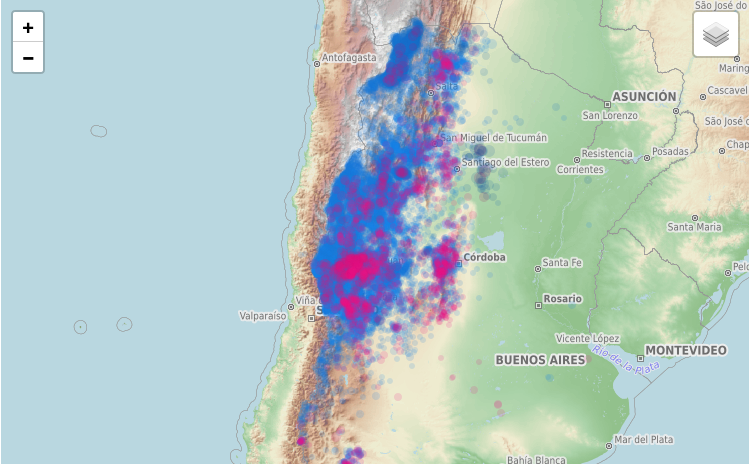
\includegraphics[width=0.8\textwidth]{mapa_sismos.png}
\caption{Los sismos no percibidos, en azul, predominan pero la mayoría se registran en zonas de montaña o cerros en su mayoría alejados de las mayores urbanizaciones.
Reproducido de \cite{daniela_parada_ic-datasets-docencia_nodate}}
\label{fig:mapa_sismos}
\end{figure}

La ubicación solo de los percibidos en un mapa político que muestra la figura \ref{fig:mapa_percibidos} muestra cierta concordancia con la figura anterior al tiempo de dejar a las claras que la percepción de los sismos por la población no es un fenómeno territorialmente homogéneo aún en provincias con abundante actividad sismica.
\begin{figure}[!h]
\centering
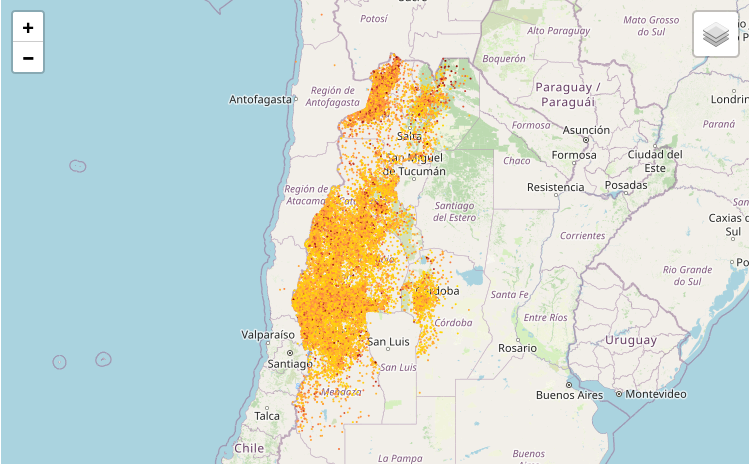
\includegraphics[width=0.8\textwidth]{mapa_percibidos.png}
\caption{Los sismos percibidos tienen una distribución poco homogénea aún en provincias con abundante actividad sismica.}
\label{fig:mapa_percibidos}
\end{figure}

De lo observado en estas figuras se hace una selección del área geográfica de los datos a trabajar que se discute en la sección siguiente.





\section{Características relevantes a la predicción}
% \section{Descripción de la selección de características (si corresponde)}

\paragraph{El problema de la distancia}
Evidentemente la proximidad de un epicentro a una población es un factor relevante en la percepción de un sismo.
El INPRES tiene una metodología operativa para registrar la ubicación de los usuarios que reportan haber percibido un sismo a través de su página web \cite{noauthor_acerca_nodate}.
Su buscador de sismos indica los sismos ``sentidos'' por usuarios con un color en sus resultados de búsqueda como ilustra la figura \ref{fig:resultado_búsqueda}.

\begin{figure}[!h]
\centering
\includegraphics[width=\textwidth]{resultado_búsqueda.png}
\caption{Resultados de una búsqueda manual de sismos en el sitio del INPRES. El indicado en rojo fue percibido por la población. En la columna \emph{intensidad} se dan datos de ubicación de la población que lo percibió.}
\label{fig:resultado_búsqueda}
\end{figure}


\paragraph{Obviando latitud y longitud}
Lamentablemente en el conjunto de datos curados no se dispone de la ubicación de la población que informó haberles percibido lo que imposibilita incorporar la distancia al epicentro como una variable en el modelo sin realizar un nuevo \emph{scrapping} de estos datos en el sitio del INPRES.
Por tal razón para este trabajo se obvian las variables de latitud y longitud del epicentro.
Para que esto no sea una factor de sesgo en el modelo se decidió filtrar por la variable ``Provincia'' y trabajar con un subconjunto de los datos que correspondan a una provincia en particular.


\paragraph{Elección de la provincia de San Juan}
Se busca que esta presente un número elevado de sismos, que tenga una extensión geográfica relativamente limitada y que el reporte de sismos percibidos no tenga sesgos geográficos, es decir una mayor preponderancia en regiones meriodionales y/o orientales que en los sentidos opuestos.
Como puede apreciarse en la figura \ref{fig:mapa_percibidos} presentada en la sección \ref{sec:AED} la provincia de San Juan cumple con estos requisitos.
Se eligió entonces la provincia de San Juan por presentar un elevado número de casos percibidos o no en el conjunto de datos, por tener una extensión geográfica reducida en comparación con otras así como contar con una alta homogeidad espacial en el reporte de sismos hace que el factor distancia entre epicentro y población que reporta tenga menor impacto que en otras provincias.
Se procedió a filtrar los datos por la provincia de San Juan con el comando \verb'sismos_SJ <- sismos[Provincia == "San Juan"]'.
Afortunadamente el subconjunto de datos de esta provincia representa un \(\approx 53 \%\) de los datos hasta aquí disponibles.
Con \num{29916} registros es aún un número suficiente para realizar un análisis de regresión logística y de clasificación con XGBoost.


\paragraph{Variables a correlacionar con la percepción}
De las originales referidas al tiempo en que se produce el terremoto \verb'Fecha' y \verb'Hora' se trabajará solo con la generada a partir de la segunda \verb'Hora_decimal' obviando la primera pues no es esperable que la percepción de un sismo por parte de la población.
De las originales referidas a la magnitud y profundidad del sismo se trabajará con la generada a partir de la primera \verb'proxy_amplitud' y la segunda sin modificación.
Quedan así un total de tres variables a trabajar en el modelo de clasificación del estado de \verb'Percibido': \verb'Hora_decimal', \verb'Profundidad' y  \verb'proxy_amplitud'.
Con la función \verb'cor' se verificó que lo covarianza de \verb'Percibido' con \verb'Hora_decimal' es casi nula, que cuanto más profundo es el terremoto es menos percibido y que \verb'proxy_amplitud' tiene ura correlación positiva, como era de esperarse, con la percepción de los sismos.
Se resume esto en el cuadro \ref{tab:correlaciones}.
\begin{table}[h]
\centering
\begin{tabular}{llll}
\toprule
\verb'Hora_decimal' & \verb'Profundidad'  & \verb'proxy_amplitud' & \verb'Percibido' \\ 
\midrule
-0.004116917  & -0.142358740  &  0.165371903 &   1.000000000 \\
\bottomrule
\end{tabular}
\caption{La fila paar la variable de percepción de la matriz de covarianza entre las variables de los sismos a analizarán muestra una débil correlación positiva con la variable que depende de la amplitud de las ondas sísmicas y una negativa con la profundidad del terremoto en concordancia con las expectaciones lógicas que pueden tenerse sobre el fenómeno.}
\label{tab:correlaciones}
\end{table}



\section{Preprocesamiento}


Las evaluaciones sobre la calidad de los modelos de clasificación generados se realizarán sobre un subconjuntos de ensayo (test) del \(20 \%\) de los datos de la provincia de San Juan, el resto se utilizará para el entrenamiento (train).

\paragraph{Escalamiento}
Previo a la partición (splitting) se realiza un escaleo uniforme sobre todo el conjunto de datos (scaling) de las tres características numéricas. 
El objeto de hacer esto previo a un ajuste lineal es que los coeficientes de la regresión sean comparables entre sí, con lo que la convergencia será más rápida y estable.
Para esto se hace uso de la función `scale` de la biblioteca `caret` para generar \verb'sismos_SJ_escalado' 


\paragraph{Partición con estratificación}
Dado el fuerte desbalance de la clase Percibido comentado en la sección \ref{sec:AED}, ante una división de los datos en subconjuntos entrenamiento y prueba estocástica está el riesgo de que el subconjunto de prueba quede con muy pocos casos positivos y no sea representativo de la distribución de la clase en el conjunto de datos. 
Para evitar esto se realiza una división estratificada de los datos en subconjuntos de entrenamiento y prueba usando la función \verb'CreateDataPartion' que indicó los índices para generar los conjuntos de datos \verb'entrenamiento_SJ' y \verb'ensayo_SJ' este último con un número aún adecuado para su función de \num{5982} registros.


\paragraph{Desbalance en entrenamiento}
Para contrarrestar el desbalance en la clase de clasificación se utilizará la técnica de sobremuestreo de la clase minoritaria que genera nuevos casos sintéticos de la clase minoritaria a partir de los existentes.
Para esto se utiliza la función \verb'ovun.sample' de la biblioteca \verb'ROSE' que genera un conjunto de datos de entrenamiento con un número de casos de la clase minoritaria igual al de la clase mayoritaria.
Se generó así un nuevo conjunto de datos de entrenamiento \verb'entrenamiento_SJ_balanceado' con \num{23934} registros.






% \section{Descripción de los métodos estadísticos utilizados (si corresponde)}



\section{Métricas de evaluación de los modelos}
% \section{Descripción de las métricas de evaluación de los modelos (si corresponde)}

Independientemente del modelo de clasificación que se utilice, la evaluación de su desempeño se realiza a partir de la comparación de las predicciones del modelo con los valores reales de la variable objetivo.
Se reservará un subconjunto de los datos para evaluar el desempeño del modelo, el conjunto de prueba y generar una matriz de confusión.

\paragraph{Matriz de confusión}
La matriz de confusión es una tabla que muestra el número de verdaderos positivos, falsos positivos, verdaderos negativos y falsos negativos del modelo.
A partir de esta matriz se pueden calcular como razones entre verdaderos y falso positivos y negativos la exactitud, precisión, sensibilidad, especificidad y el valor F1.

\paragraph{Exactitud (accuracy)}
La exactitud es la proporción de predicciones correctas sobre el total de casos.
Se calcula como
\begin{equation}
	\text{Exactitud} = \frac{\text{Verdaderos positivos} + \text{Verdaderos negativos}}{\text{Verdaderos pos} + \text{Falsos pos} + \text{Verdaderos neg} + \text{Falsos neg}}.
\end{equation}

\paragraph{Precisión}
La precisión es la proporción de predicciones correctas sobre el total de predicciones realizadas.
Se calcula como
\begin{equation}
	\text{Precisión} = \frac{\text{Verdaderos positivos} + \text{Verdaderos negativos}}{\text{Verdaderos pos} + \text{Falsos pos} + \text{Verdaderos neg} + \text{Falsos neg}}.
\end{equation}

\paragraph{Sensibilidad (recall)}
La sensibilidad es la proporción de verdaderos positivos sobre el total de casos positivos.
Se calcula como
\begin{equation}
	\text{Sensibilidad} = \frac{\text{Verdaderos positivos}}{\text{Verdaderos positivos} + \text{Falsos negativos}}.
\end{equation}

\paragraph{Especificidad}
La especificidad es la proporción de verdaderos negativos sobre el total de casos negativos.
Se calcula como
\begin{equation}
	\text{Especificidad} = \frac{\text{Verdaderos negativos}}{\text{Verdaderos negativos} + \text{Falsos positivos}}.
\end{equation}

\paragraph{F1-score}
El \emph{F1-score} es la media armónica de la precisión y la sensibilidad (recall).
Se calcula como
\begin{equation}
	\text{F1-score} = 2 \times \frac{\text{Precisión} \times \text{Recall}}{\text{Precisión} + \text{Recall}}.
\end{equation}

Con un grafico de estas métricas en función del punto de corte entre clases se elige manualmente este que permita clasificar las instancias en una de las dos clases.

Como complemento se pueden trazar las curvas ROC y PR para evaluar el desempeño de los modelos en separar las clases.

\paragraph{Área bajo la curva ROC}
El área bajo la curva ROC (AUC-ROC) es una métrica que evalúa la capacidad de un modelo de clasificación para discriminar entre clases.
Se calcula como el área bajo la curva ROC, que es la curva que representa la tasa de verdaderos positivos en función de la tasa de falsos positivos.
El valor de AUC-ROC varía entre 0 y 1, donde 0 indica un modelo que clasifica todas las instancias de la clase positiva como negativas y viceversa, y 1 indica un modelo que clasifica perfectamente las instancias de ambas clases.

\paragraph{Área bajo la curva PR}
El área bajo la curva PR (AUC-PR) es una métrica que evalúa la capacidad de un modelo de clasificación para discriminar entre clases.
Se calcula como el área bajo la curva PR, que es la curva que representa la precisión en función del \emph{recall}.
El valor de AUC-PR varía entre 0 y 1, donde 0 indica un modelo que clasifica todas las instancias de la clase positiva como negativas y viceversa, y 1 indica un modelo que clasifica perfectamente las instancias de ambas clases.

%\paragraph{Validación cruzada}
%La validación cruzada es una técnica que se utiliza para evaluar el desempeño de un modelo de clasificación.
%Consiste en dividir el conjunto de datos en \(k\) subconjuntos, entrenar el modelo en \(k-1\) subconjuntos y evaluarlo en el subconjunto restante.
%Este proceso se repite \(k\) veces, de modo que cada subconjunto se utiliza una vez como conjunto de prueba.
%

% En este trabajo se utilizará la AUC-ROC la utilizada para de los modelos de clasificación ajustados en este trabajo.

\chapter{Resultados y discusión}

\section{Presentación de resultados}
% \section{Presentación y análisis de resultados obtenidos}

\subsection{Predictor por regresión logística}

\subsubsection*{Múltiple sin interacción entre variables}

El primer modelo ensayado es uno múltiple de regresión logística con las variables \verb'Hora_decimal', \verb'Profundidad' y \verb'proxy_amplitud' como predictores sin interacción entre ellos,

\begin{align}
	\log \left( \frac{p}{1-p} \right) = &
	 \beta_0 + \beta_1\, \text{Hora\_decimal} + \beta_2 \, \text{Profundidad}\notag\\
	& + \beta_3 \, \text{proxy\_amplitud},
	\label{eq:regresion_logistica}
\end{align}

La función \verb'summary' produce un resumen de los resultados arroja para los coeficientes:
\begin{verbatim}
	Coefficients:
                Estimate Std. Error z value Pr(>|z|)    
(Intercept)    -0.311098   0.014614 -21.287   <2e-16 ***
Hora_decimal   -0.015398   0.013362  -1.152    0.249    
Profundidad    -0.555176   0.010705 -51.863   <2e-16 ***
proxy_amplitud  0.167536   0.006263  26.750   <2e-16 ***
\end{verbatim} 
Esto indica que excepto el coeficiente \(\beta_1\) para la \verb'Hora_decimal', todos son significativos ya que sus probabilidades de que no tengan esos valores y se cumpla la hipótesis nula \(Pr(>|z|)\) para el estadístico \(z = \frac{\beta}{\sigma_\beta}\) se indican como muy inferiores a \(0.05\).

Para definir el punto de corte entre las clases se graficaron las métricas de evaluación en función de este como ilustra la figura \ref{fig:múltiple_metrics}.
Si en base a la inspección de esa figura eligiera el punto de corte en \(0.5\) se obtendrían las métricas de evaluación que se resumen en la tabla \ref{tab:múltiple_metrics}.

\begin{figure}[!h]
	\centering
	\input{graphs/múltiple_metrics.tex}
	\caption{Métricas de evaluación para definir manualmente el punto de corte entre clases para el modelo de regresión logística múltiple sin interacción entre variables.}
	\label{fig:múltiple_metrics}
\end{figure}

\begin{table}[h]
\centering
\begin{tabular}{lllll}
\toprule
corte & exactitud & sensitividad & especificidad & precisión \\
\midrule
\num{0.5} & \num{0.8726179} & \num{0.5365854} & \num{0.8796723} & \num{0.08560311} \\
\bottomrule
\end{tabular}
\caption{Métricas de evaluación para el modelo de regresión logística múltiple sin interacción entre variables con punto de corte en \(0.5\).}
\label{tab:múltiple_metrics}
\end{table}


Continuando con el análisis de la regresión logística ahora vería si logro mejorar estas métricas con un modelo que incluya interacción entre las variables.

\subsubsection{Múltiple con interacción entre variables}
\textcolor{red}{Esto es un placeholder para una sección aún vacía.}


\subsection{Predictor por XGBoost}
\textcolor{red}{Esto es un placeholder para una sección aún vacía.}



\section{Relevancia de los resultados}
% \section{Discusión de los resultados y su relevancia}
\textcolor{red}{Esto es un placeholder para una sección aún vacía.}



\section{Limitaciones y posibles mejoras}
\textcolor{red}{Esto es un placeholder para una sección aún vacía.}




\chapter{Conclusión}

\section{Resumen de los hallazgos principales}
\textcolor{red}{Esto es un placeholder para una sección aún vacía.}



\section{Conclusiones generales y su relación con los objetivos del trabajo}
\textcolor{red}{Esto es un placeholder para una sección aún vacía.}



\section{Aplicaciones y relevancia de los resultados}
\textcolor{red}{Esto es un placeholder para una sección aún vacía.}



% \backmatter

%% bibliografía
% \printbibliography[heading=bibnumbered] % numbered as chapter
\printbibliography[heading=bibintoc] % not numbered

% Bibliografía:
% Referencias bibliográficas citadas en el documento
% Otras fuentes consultadas


\chapter*{Anexos (opcionales)}
\addcontentsline{toc}{chapter}{Anexos (opcionales)}


\section{Código fuente utilizado en el análisis}
Enlace al \href{https://github.com/bettachini/tallerTesis/tree/main/sismosURL}{repositorio en GitHub} que aloja el código fuente utilizado en el análisis de los datos.
% \textcolor{red}{Esto es un placeholder para una sección aún vacía.}



\section{Tablas y gráficos adicionales}
\textcolor{red}{Esto es un placeholder para una sección aún vacía.}


\section{Otros materiales relevantes}
\textcolor{red}{Esto es un placeholder para una sección aún vacía.}


\end{document}